\documentclass[11pt, oneside]{book}
\usepackage{geometry}
\geometry{letterpaper}
\usepackage[parfill]{parskip}
\usepackage{graphicx}

\usepackage{amsmath}
\usepackage{amsfonts}
\usepackage{amssymb}
\usepackage{pgfplots}
\pgfplotsset{compat=newest}

% Essential Packages
\usepackage{ragged2e}
\usepackage{amssymb}
\usepackage{amsmath}
\usepackage{mathrsfs}
\usepackage[utf8]{inputenc}
\usepackage[english]{babel}
\usepackage[hyperref]{ntheorem}

% Theorem Style Customization
\setlength\theorempreskipamount{2ex}
\setlength\theorempostskipamount{3ex}

% hyperref Package Settings
\usepackage{hyperref}
\hypersetup{
	colorlinks = true,
	linkcolor = magenta
}

% ntheorem Declarations
\theoremstyle{break}
\newtheorem{thm}{Theorem}[section]
\newtheorem*{proof}{Proof}
%\newtheorem{crly}{Corollary}[section]
\newtheorem{lemma}{Lemma}[section]
\newtheorem{propo}{Proposition}[section]
\newtheorem{claim}{Claim}[section]
\newtheorem*{remark}{Remark}
\newtheorem*{note}{Note}
\newtheorem{defn}{Definition}[section]
\newtheorem{eg}{Example}[section]
\newtheorem{ex}{Exercise}[section]
\newtheorem{cor}{Corollary}[section]

\newcommand{\cA}{ {\cal A} }
\newcommand{\fA}{ {\mathfrak{A}} }
\newcommand{\cB}{ {\cal B} }
\newcommand{\cD}{ {\cal D} }
\newcommand{\cF}{ {\cal F} }
\newcommand{\cL}{ {\cal L} }

\newcommand{\bA}{ {\mathbb{A}} }
\newcommand{\bC}{ {\mathbb{C}} }
\newcommand{\bF}{ {\mathbb{F}} }
\newcommand{\bN}{ {\mathbb{N}} }
\newcommand{\bQ}{ {\mathbb{Q}} }
\newcommand{\bR}{ {\mathbb{R}} }
\newcommand{\bZ}{ {\mathbb{Z}} }
\newcommand{\bP}{ {\mathbb{P}} }
\newcommand{\bo}{ {\mathcal{O}} }
\newcommand{\bbc}{ {\mathcal{C}} }


\newcommand{\ba}{ \vec{a} }
\newcommand{\bb}{ \vec{b} }
\newcommand{\pp}{ \vec{p} }
\newcommand{\qq}{ \vec{q} }
\newcommand{\ts}{ \vec{s} }
\newcommand{\uu}{ \vec{u} }
\newcommand{\vv}{ \vec{v} }
\newcommand{\xx}{ \vec{x} }
\newcommand{\yy}{ \vec{y} }
\newcommand{\zz}{ \vec{z} }
\newcommand{\zv}{ \vec{0} }

\newcommand{\aks}{ ( \, \ba_k \, )_{k=1}^{\infty} }
\newcommand{\xks}{ ( \, \xx_k \, )_{k=1}^{\infty} }
\newcommand{\yks}{ ( \, \yy_k \, )_{k=1}^{\infty} }
\newcommand{\qks}{ ( q_k )_{k=1}^{\infty} }
\newcommand{\tks}{ ( t_k )_{k=1}^{\infty} }

\newcommand{\limk}{ \lim_{k \to \infty} }
\newcommand{\ee}{ \varepsilon }
\newcommand{\limi}{ \lim_{i \to \infty} }

\providecommand*{\axiomautorefname}{Axiom}
\providecommand*{\lemmaautorefname}{Lemma}
\providecommand*{\thmautorefname}{Theorem}
\providecommand*{\propoautorefname}{Proposition}

% ntheorem listtheorem style
\makeatletter
\def\thm@@thmline@name#1#2#3#4{%
        \@dottedtocline{-2}{0em}{2.3em}%
                   {\makebox[\widesttheorem][l]{#1 \protect\numberline{#2}}#3}%
                   {#4}}
\@ifpackageloaded{hyperref}{
\def\thm@@thmline@name#1#2#3#4#5{%
    \ifx\#5\%
        \@dottedtocline{-2}{0em}{2.3em}%
            {\makebox[\widesttheorem][l]{#1 \protect\numberline{#2}}#3}%
            {#4}
    \else
        \ifHy@linktocpage\relax\relax
            \@dottedtocline{-2}{0em}{2.3em}%
                {\makebox[\widesttheorem][l]{#1 \protect\numberline{#2}}#3}%
                {\hyper@linkstart{link}{#5}{#4}\hyper@linkend}%
        \else
            \@dottedtocline{-2}{0em}{2.3em}%
                {\hyper@linkstart{link}{#5}%
                  {\makebox[\widesttheorem][l]{#1 \protect\numberline{#2}}#3}\hyper@linkend}%
                    {#4}%
        \fi
    \fi}
}
\makeatother
\newlength\widesttheorem
\AtBeginDocument{
  \settowidth{\widesttheorem}{Proposition A.1.1.1\quad}
}

\theoremlisttype{allname}

% Shortcuts
%\newcommand{\bb}[1]{\mathbb{#1}}			% using bb instead of mathbb
\newcommand{\floor}[1]{\lfloor #1 \rfloor}	% simplifying the writing of a floor function
\newcommand{\ceiling}[1]{\lceil #1 \rceil}	% simplifying the writing of a ceiling function
\newcommand{\dotp}{\, \cdotp}				% dot product to distinguish from \cdot

% Custom math operator
\DeclareMathOperator{\rem}{rem}
\DeclareMathOperator{\id}{id}
\DeclareMathOperator{\order}{order}

% Main Body
\title{CO 367 - Nonlinear Optimization (Class Notes)}
\author{Saiyue Lyu}

\begin{document}
\hypersetup{pageanchor=false}
\maketitle
\hypersetup{pageanchor=true}
\tableofcontents

\chapter*{List of Definitions}
\theoremlisttype{all}
\listtheorems{defn}



\chapter{Introduction}

Mathematical Optimization (formally math programming)

Find a best soln to the model of a problem

{\bf Application : }

$\bullet$ Operation Research

\hspace{1cm} 1) Scheduling and Planning

\hspace{1cm} 2) Supply Chain Management

\hspace{1cm} 3) Vehicle Routing

\hspace{1cm} 4) Power Grid Optimization

$\bullet$ Statistics and Machine Learning

\hspace{1cm} 1) Curve Fitting

\hspace{1cm} 2) Classification, Clustering, SVM ...

\hspace{1cm} 3) Deep Learning

$\bullet$ Finance

$\bullet$ Optimal Control

$\bullet$ Biology -- Protein Folding

\newpage

Optimization

\begin{equation*}
\begin{aligned}
(OPT)& \underset{X}{\text{minimize}}
& & f(x) & & \mbox{ objective function}\\
& \text{subject to}
& & g_i(x)\leq 0, \; \forall i=1,\cdots,m & &\mbox{ constraints}\\
&&& x \in\bR^n .
\end{aligned}
\end{equation*}

\remark

1) $\max f(x) =-\min -f(x)$

2) $\{ x\in\bR^n, g(x)\geq 0\}=\{x\in\bR^n, -g(x)\leq 0\}$

3) $\{x\in\bR^n, g(x)\leq b\}=\{x\in\bR^n, g(x)-b\leq 0\}$

\section{Classification of Solns}
\defn[Open ball \& Closure] The open ball of radius $\delta$ around $\bar{x}$ is $B_{\delta}(\bar{x})=\{x\in\bR^n, ||x-\bar{x}||<\delta\}$ 

The closure of $B_{\delta}(\bar{x})$ is $\overline{B_{\delta}}(\bar{x})=\{x\in\bR^n, ||x-\bar{x}||\leq \delta\}$

\defn[Global \& Local Minimizer] Consider $f: D\to \bR$. the point $x^*\in D$ is 

$\bullet$ a global minimizer for $f$ on $D$ if $f(x^*)\leq f(x),\forall x\in D$

$\bullet$ a strict global minimizer for $f$ on $D$ if $f(x^*)< f(x),\forall x\in D, x\neq x^*$

$\bullet$ a local minimizer for $f$ on $D$ if $\exists \delta>0, f(x^*)\leq f(x),\forall x\in B_{\delta}(x^*)\cap D$

$\bullet$ a strict local minimizer for $f$ on $D$ if $\exists \delta>0, f(x^*)< f(x),\forall x\in B_{\delta}(x^*)\cap D, x\neq x^*$

\section{Classification of Problems}
1. If $f(x)=0, \forall x\in \bR^n$, then (OPT) is a feasible problem

2. If we have $m=0$ constraints, then (OPT) is an unconstrained optimization problem.

\section{Classification of Problems -- Types of functions involved}

Why do we care?

In the absence of hypothesis on $f$ and $g$, (OPT) is unsovlable.

\note "Black box" optimization framework.

All we have is an "oracle" that can compute values of $f(x)$ for any $x$ (and possibly some derivatives)

\eg Consider $h(x)=\begin{cases}
    0,& \text{if } x\in\bZ^n\\
    1,              & \text{otherwise}
\end{cases}$
\begin{equation*}
\begin{aligned}
& \underset{X}{\text{minimize}}
& & f(x) \\
& \text{subject to}
& & g_i(x)\leq 0, \; \forall i=1,\cdots,m \\
&&& h(x)\leq 0,\\
&&& x \in\bR^n .
\end{aligned}
\end{equation*}

In other word, we want $x\in\bZ^n$, where $\bZ^n$ is a lattice

\defn[discrete optimization problem]
When the constraints of (OPT) restrict solns to a lattice, then (OPT) is called a discrete optimization problem

\defn[Continuous Function]
A function $f: D\to \bR$ is continuous over $D$ if $\forall \epsilon>0, \exists \delta>0$ such that $|x-y|<\delta\,\Leftarrow\,|f(x)-f(y)|<\epsilon,\forall x,y\in D$

\defn[$C^k$-smooth]
A function $f:D\to\bR$, $D\subset \bR^n$ is open, then $f$ is $C^k$-smooth over $D$ \big(i.e. $f\in C^k(D)$\big) if all its $\leq k$-th derivatives are continuous over $D$

\eg  

$h(x)=\begin{cases}
    1,& \text{if } x\geq 2\\
    -1,& \text{if } x< 2            
\end{cases}$ is discontinuous

$g(x)=|x-2|$ is continuous and $C^0$ smooth

$f(x)=\begin{cases}
    \frac{1}{2}(x-2)^2,& \text{if } x\geq 2\\
    \frac{1}{@}(2-x)^2,& \text{if } x< 2            
\end{cases}$ is continuous and $C^1$ smooth

\defn[Gradient]
Let $f\in C^1(D)$ for some $D\subset \bR^n$. Its Gradient $\nabla f\in C^0(D): D\to \bR^n$ is given by 
\begin{center}
    $\nabla f(x)=\begin{bmatrix}
    \frac{\partial f}{\partial x_1}(x)\\
    \vdots
    \frac{\partial f}{\partial x_n}(x)\\
    \end{bmatrix}$
\end{center}

\defn[Hessian]
Let $f\in C^2(D)$ for some $D\subset \bR^n$. Its Hessian $\nabla^2 f\in C^1(D): D\to \bR^{n\times n}$ is given by 
\begin{center}
    $\nabla^2 f(x)=\begin{bmatrix}
    \frac{\partial f}{\partial x_1\partial x_1}(x)  & \dots  &  \frac{\partial f}{\partial x_1\partial x_n}(x)\\
    \vdots  & \ddots & \vdots \\
     \frac{\partial f}{\partial x_n\partial x_1}(x)  & \dots  &  \frac{\partial f}{\partial x_n\partial x_n}(x)
\end{bmatrix}$
\end{center}

\remark
If $f$ and $g$ are linear functions, then (OPT) is a linear programming problem.


\chapter{Linear Algebra}
\section{Vector and Matrix Norm}
\defn[Norm]
A norm $||\cdot||$ on $\bR^n$ assigns a scalar $||x||$ to every $x\in\bR^n$ such that

1) $||x||\geq 0,\forall x\in\bR^n$

2) $||c\cdot x||=|c|\cdot||x|\,\forall c\in\bR, x\in\bR^n$

3) $||x||=0\Longleftrightarrow x=0$

4) $||x+y||\leq ||x||+||y||$

\begin{remark}
\begin{align*}
    &L^k Norm & ||x||_k=(\sum_{i=1}^n|x_i|^k)^{1/k}\\
    &Manhattan Norm  & ||x||_1=\sum|x_i|\\
    &Euclidean Norm & ||x||_2=\sqrt{\sum x_i^2}\\
    &Infinite Norm & ||x||_{\infty}=\max |x_i|
\end{align*}
\end{remark}

\begin{thm}[Schwartz Inequality]
$\forall x,y\in\bR^n, |x^Ty|\leq ||x||_2\cdot||y||_2$, the equality holds when $x=\lambda y$ for some $\lambda\in\bR$
\end{thm}

\begin{thm}[Pythagorean Thm]
If $x,y\in\bR^n$ are orthogonal, then $||x+y||_2^2=||x||_2^2+||y||_2^2$
\end{thm}

\begin{defn}[Induced Norm]
Given a vector norm $||\cdot||$, the induced matrix norm associates a scalar $||A||$ to all $A\in\bR^{n \times n}$ with $||A||=\displaystyle\max_{||x||=1}||Ax||$
\end{defn}

\begin{propo}
$||A||_2=\displaystyle\max_{||x||_2=1}||Ax||_2=\displaystyle\max_{||x||_2=||y||_2=1}|y^TAx|$
\begin{proof}
Apply Schwartz Inequality to $|y^TAx|$
\end{proof}
\end{propo}

\begin{propo}
$||A||_2=||A^T||_2$
\begin{proof}
Swap $x$ and $y$ in the above Proposition 2.1.1
\end{proof}
\end{propo}

\begin{propo}
Let $A\in\bR^{n \times n}$, TFAE:

1) $A$ is nonsingular

2) $A^T$ is nonsingular

3) $\forall x\in \bR^n\setminus\{0\}, Ax\neq 0$

4) $\forall b\in\bR^n, \exists x\in\bR^n$ unique such that $Ax=b$

5) Columns of $A$ are linear independent

6) Rows of $A$ are linearly independent

7) $\exists B\in\bR^{n \times n}$ unique such that $AB=I=BA$, where $B$ is the inverse of $A$

8) $\forall A,B\in\bR^{n \times n}, (AB)^{-1}=B^{-1}A^{-1}$ if $B^{-1}$ exists
\end{propo}

\section{Eigenvalues}

\defn[Eigenvalue \& Eigenvector]
The characteristic polynomial $\phi : \bR\to\bR$ of $A\in\bR^{n \times n}$ is $\phi(\lambda)=\det(A-\lambda I)$. It has $n$ (possibly complex or repeated) roots, which are the eigenvalues of $A$. Given an eigenvalue $\lambda$ of $A$, $x\in\bR^n$ is the corresponding eigenvector of $A$ if $Ax=\lambda x$

\propo
Given $A\in\bR^{n\times n}$

1) $\lambda$ is an eigenvalue $\Longleftrightarrow$
 $\exists$ a corresponding eigenvector
 
2) $A$ is singular $\Longleftrightarrow$ it has a zero eigenvector

3) If $A$ is triangular, then its eigenvector are its diagonal entries

4) If $S\in\bR^{n\times n}$ is nonsingular and $B=SAS^{-1}$, then $A,B$ have the same eigenvalues

5) If the eigenvalues of $A$ are $\lambda_1,\cdots,\lambda_n$, then 

\hspace{0.5cm} $\bullet$ the eigenvalues of $A+cI$ are $\lambda_1+c,\cdots,\lambda_n+c$

\hspace{0.5cm} $\bullet$ the eigenvalues of $A^k$ are $\lambda_1^k,\cdots,\lambda_n^k, k\in\bR$

\hspace{0.5cm} $\bullet$ the eigenvalues of $A^{-1}$ are $\frac{1}{\lambda_1},\cdots,\frac{1}{\lambda_n}$

\hspace{0.5cm} $\bullet$ the eigenvalues of $A^T$ are $\lambda_1,\cdots,\lambda_n$

\defn[Spectral Radius]
The spectral radius of $\rho(A)$ of $A\in\bR^{n\times n}$ is $\displaystyle\max_{\lambda \mbox{ is eigenvalue}}|\lambda|$

\propo
For any induced norm $||\cdot||, \rho(A)\leq ||A^k||^{1/k}$ for $k=1,2,\cdots$
\begin{proof}
{\bf Trick : } $||A^k||=\displaystyle\max_{||y||=1}||A^ky||=\displaystyle\max_{y\neq 0}\frac{1}{||y||}||A^ky||$

In particular, let $\lambda$ be any eigenvalue of $A$, $x$ be the corresponding eigenvector
\begin{align*}
    ||A^k||\geq \frac{1}{||x||}||A^k\cdot x||&=\frac{1}{||x||}||A\cdots A\cdot x||\\
    &=\frac{1}{||x||}||\lambda^k \cdot x||\\
    &=|\lambda^k|
\end{align*}

So for any eigenvalue $\lambda, ||A^k||\geq |\lambda|^k$

Therefore $||A^k||^{1/k}\geq |\lambda|, \forall \lambda$, thus $||A^k||^{1/k}\geq \rho(A)$
\end{proof}

\propo
For any induced norm $||\cdot||, \displaystyle\lim_{k\to\infty}||A^k||^{1/k}=\rho(A)$
\proof Too long, omitted


\section{Symmetric Matrices}

\propo
Let $A\in\bR^{n\times n}$ be symmetric, then

1) Its eigenvalues are all $\bR$eal

2) Its eigenvetors are $n$ mutually orthogonal $\bR$eal nonzero vectors

3) If the $n$ eigenvectors $x_1,\cdots,x_n\in\bR^n$ are normalized such that $||x||_2=1$ with corresponding eigenvalues $\lambda_1,\cdots,\lambda_n$, then $A=\sum_{i=1}^n\lambda_i x_i x_i^T$
\proof  Easy

\propo
Let $A\in\bR^{n\times n}$ be symmetric, then $||A||_2=\rho(A)$
\proof
We already know $\rho(A)\leq ||A^k||^{1/k}$, in particular, $\rho(A)\leq ||A||_2$

It remains to show that $\rho(A)\geq ||A||_2$

Because the eigenvectors $x_i, i=1,\cdots,n$ of $A$ can be assumed ,utually orthogonal

Then we can write any $y\in\bR^n$ as $y=\sum_{i=1}^n \beta_i x_i$ for some $\beta_i\in\bR$

By Pythagorean Thm, $||y||_2^2=\sum\beta_i^2||x_i||_2^2$

Now $Ay=A\sum\beta_i x_i=\sum\beta_iA x_i=\sum\beta_i\lambda_ix_i$

Since all $x_i$ are mutually orthogonal, by Pthahorean Thm again, have
\begin{align*}
    ||Ay||_2^2&=\sum\beta_i^2\lambda_i^2||x_i||_2^2\\
    &\leq \sum\beta_i^2\rho(A)^2||x_i||_2^2\\
    &=\rho(A)^2||y||_2^2
\end{align*}

By which we get, $||Ay||_2\leq \rho(A)||y||_2$

Also by the definition, we have
\begin{align*}
    ||A||_2&=\displaystyle\max_{y\neq 0}\frac{1}{||y||_2}||Ay||_2\\
    &\leq \displaystyle\max_{y\neq 0}\frac{1}{||y||_2}\cdot\rho(A)||y||_2\\
    &=\rho(A)
\end{align*}

\begin{propo}
Let $A\in\bR^{n\times n}$ be symmetric with eigenvalues $\lambda_1,\cdots,\lambda_n\in\bR$

Then $\forall y\in\bR^n, \lambda_1||y||_2^2\leq y^TAy\leq \lambda_n||y||_2^2$
\begin{proof}
Again, write $y=\sum \beta_i x_i$ for some $\beta_i\in\bR$ with $x_i$ are the orthogonal eigenvectors

On the one hand,
\begin{align*}
    y^TAy&=(\sum\beta_i x_i)^T(\sum\beta_i \lambda_ix_i)\\
    &=\sum\beta_i^2\lambda_ix_i^Tx_i\mbox{ as }x_ix_j=0\mbox{ if }i\neq j\\
    &=\sum\beta_i^2\lambda_i||x_i||_2^2
\end{align*}

WLOG, we can assume $||x_i||_2=1$, then we have 
\begin{align*}
    y^TAy=\sum\beta_i^2\lambda_i
\end{align*}

On the other hand,
\begin{align*}
    ||y||_2^2=\sum\beta_i^2||x_i||_2^2=\sum\beta_i^2
\end{align*}

Clearly, we have 
\begin{align*}
    \lambda_1\sum\beta_i& &\leq& & \sum\beta_i^2\lambda_i& &\leq & & \lambda_n\sum\beta_i^2\\
    \lambda_1||y||_2^2& &\leq&  &y^TAy & &\leq &&\lambda_n||y||_2^2
\end{align*}
\end{proof}

\remark {\bf Why can we assume $||x_i||_1=1$? }

As $x_i$ being the eigenvectors of $A$ are defined up to scalar $Ax=\lambda x$, we have 
\begin{center}
 $A(\frac{1}{||x||}x)=\lambda(\frac{1}{||x||}x)$   
\end{center}
\end{propo}

\propo
Let $A\in\bR^{n\times n}$ be symmetric, then $||A^k||_2=||A||_2^k,\forall k=1,2,\cdots$
\begin{proof}
Since $A^T=A$, then $(A^k)^T=(A\cdots A)^T=A^T\cdots A^T=A\cdots A=A^k$

Since $A^k$ is symmetric, then $||A^k||_2=\rho(A^k)$

We know that the eigenvalues of $A^k$ are $\lambda_1^k,\cdots,\lambda_n^k$

Thus $\rho(A^k)=\big(\rho(A)\big)^k$

We know $\rho(A)=||A||_2$, therefore $||A||_2^k=||A^k||_2$
\end{proof}

\propo 
Let $A\in \bR^{n\times n}$ (not necessary symmetric), then $||A||_2^2=||A^TA||_2=||AA^T||_2$
\begin{proof}

On the one hand,

$||Ax||_2^2=(Ax)^T(Ax)=x^T(A^TAx)\leq ||x||_2\cdot||A^TAx||_2\leq ||x||_2\cdot||AA^T||_2\cdot||x||_2$

$||A||_2^2=\displaystyle\max_{x\in\bR^n} \frac{1}{||x||_2^2}\cdot||Ax||_2^2\leq||A^TA||_2$

On the other hand,
\begin{align*}
||A^TA||&=\displaystyle\max_{||x||=||y||=1} |y^T A^T Ax|\\
    &\leq\displaystyle\max_{||y||=1,||x||=1} ||y^TA^T||_2\cdot||Ax||_2\mbox{ by CS ineq}\\
    &=\big(\displaystyle\max_{||y||=1} ||y^TA^T||_2\big)\big(\displaystyle\max_{||x||=1}||Ax||_2\big)\\
    &=||A||_2\cdot||A||_2\\
    &=||A||_2^2
\end{align*}

Combine these two things, we get $||A||_2^2=||A^TA||_2$

For the other equality, swap $A$ and $A^T$ in the proof and use $||A||_2=||A^T||_2$
\end{proof}

\propo

$||A^{-1}||_2$ is $\frac{1}{|\lambda_1|}$, where $\lambda_1$ is the smallest magnitude eigenvalue of $A$
\begin{proof}
We know $||A^{-1}||_2=\rho(A^{-1})$, and the eigenvalues of $A^{-1}$ are the inverse of the eigenvalues of $A$
\end{proof}

\section{Positive Definite Matrices}
\defn[Positive Definite \& Positive Semidefinite]
A symmetric matrix $A\in\bR^{n\times n}$ is positive definite if $x^TAx>0,\forall x\in\bR^n, x\neq 0$, it is positive semidefinite if $x^TAx\geq 0,\forall x\in\bR^n$

\note 

pd. for symmetric positive definite, psd. for symmetric positive semidefinite

\propo
For any $A\in\bR^{n\times n}$(possibly non square), $A^TA$ is psd. Then the matrix $A^TA$ is pd iff $A$ has full column rank (i.e. $rank(A)=n$; which implies $m\geq n$)

\begin{proof}
1) $A^TA$ is square and symmetric (immediate)

2) $A^TA$ is psd. : $\forall x\in\bR^n, x^T(A^TA)x=(Ax^T)(Ax)=||Ax||_2^2\geq 0$

3) pd. iff $rank(A)=n$ : 
\begin{align*}
    &x^TA^TAx>0,\forall x\in bE^n, x\neq 0\\
    \Longleftrightarrow &||Ax||_2^2>0\\
    \Longleftrightarrow &||Ax||_2>0\\
    \Longleftrightarrow &Ax\neq 0, \forall x\in\bR^n, x\neq 0\\
    \Longleftrightarrow &\mbox{ the columns of $A$ are linearly independent}\\
    \Longleftrightarrow &rank(A)=n
\end{align*}
\end{proof}

\cor 
If $A\in\bR^{n\times n}$ is square, then $A^TA$ is pd. iff $A$ is nonsingular

\propo 
A square symmetric matrix is psd. (rsp pd.) iff all its eigenvalues are $\geq 0$ (rsp $>0$)
\begin{proof}
We will prove the statement for psd/$\geq 0$, the proof is similar for pd/(>0)

($\Rightarrow$) Let  $\lambda$ be an eigenvalue of $A$ psd. and let $x$ be the corresponding nonzero eigenvector

\hspace{0.5cm}
Then $x^tAx\geq 0$, so $x^T\lambda x=\lambda||x||_2^2\geq 0$

\hspace{0.5cm}
Thus $\lambda\geq 0$

($\Leftarrow$) Let $\lambda_1,\cdots,\lambda_n$ be the eigenvalues of $A$ and let $x_1,\cdots,x_n$ be the n (nonzero, real, mutually orthogonal) eigenvectors.

\hspace{0.5cm}
For any $y\in\bR^n$, we can write 
\begin{center}
    $y=\sum \beta_i x_i$ for some $\beta_i\in\bR$
\end{center}

\hspace{0.5cm}
Then we have 
\begin{align*}
    y^TAy&=(\sum \beta_i x_i)^T\cdot A\cdot (\sum \beta_i x_i)\\
    &=(\sum \beta_i x_i)^T(\sum\beta_i Ax_i)\\
    &=(\sum \beta_i x_i)^T(\sum \beta_i \lambda_ix_i)\\
    &=\sum\beta_i^2\lambda_i||x_i||_2^2\mbox{ as $x_i$ are orthogonal}\\
    &\geq 0
\end{align*}
\end{proof}

\propo 
The inverse of a pd. matrix is pd.
\begin{proof}
Let $\lambda_1,\cdots,\lambda_n>0$ be the eigenvalues of $A$ pd. 

Then the eigenvalues of $A^{-1}$ are $\frac{1}{\lambda_1},\cdots,\frac{1}{\lambda_n}$
\end{proof}

\chapter{Convexity}

\section{Basic Intro}

\defn[Convex Set]
A set $C\subset \bR^n$ is convex if $\lambda x+(1-\lambda)y\in C,\forall x,y\in C, \forall 0\leq \lambda\leq 1$

\eg The set of two disjoint sets is nonconvex

A "donut" is nonconvex

\defn[Convex Function]
Let $D\subset\bR^n$ be a convex set, a function $f : D\to \bR$ is sid to be convex if $f\big(\lambda x+(1-\lambda)y\big)\leq \lambda f(x)+(1-\lambda)f(y), \forall x,y\in D, \forall 0\leq \lambda\leq 1$

A function is said to be strict convex if a strict inequality ($<$) holds as well

\eg $y=x^2$ is a convex function,  \hspace{1cm} $y=-x^2$ is non-convex (concave)

\propo 
1) For any collection of $\{C_i :i\in I\}$ of convex sets, their intersection $\displaystyle\cap_{i\in I} C_i$ is convex

2) The vector (Minkowski) sum $\{x+y : x\in C_1, y\in C_2\}$ of two convex sets $C_1, C_2$ is convex

3) The image of a convex set under a linear transformation is a convex set

\defn[Level Set \& Epigraph]
Let $f: D\to \bR$ be a function with $D$ convex, 

The level sets of $f$ are $\{x\in D: f(x)\leq\alpha\}$ for all $\alpha\in\bR$ (sometimes $"<"$)

The epigraph of $f$ is s subset of $\bR^{n+1}$ given by $epi(f)=\{(x,\alpha), x\in D, \alpha\in\bR,f(x)\leq \alpha\}$

\propo
1) If $f: D\to\bR$ is convex, then its level sets are convex as well

2) $f:D\to\bR$ is convex iff its epigraph is a convex set

\note The converse of 1) is not true ! For example, $f(x)=\sqrt{|x|}$

The level sets of $f$ is $\sqrt{|x|}\leq\alpha\Longleftrightarrow|x|\leq\alpha^2\Longleftrightarrow\alpha^2\leq x\leq \alpha^2$

However, $f$ is not convex !

\propo
1) Any linear function is convex (but not strictly convex)

2) If $f$ is a convex function, then $g(x)=\lambda f(x)$ is convex for all $\lambda\geq 0$

3) The sum of two convex functions is a convex function

4) The maximum of two convex functions is a convex function (does not work for minimum)

\propo
Any vector norm is convex (this is useful as optimize convex function is usually possible)
\begin{proof}
Let $f(x)=||x||$, then $\forall x,y\in\bR^n,0\leq \lambda\leq 1$, have 
\begin{align*}
    f\big(\lambda x+(1-\lambda)y\big)&=||\lambda x+(1-\lambda)y||\\
    &\leq ||\lambda x||+||(1-\lambda)y||\\
    &=\lambda\cdot ||x||+(1-\lambda)\cdot ||y||\\
    &=\lambda f(x)+(1-\lambda) f(y)
\end{align*}
\end{proof}

\section{Taloy's Thms}

\thm[Talor's Thm For Uni-variate Functions]
$f(x+h)=\sum_{i=0}^k\frac{h^i}{i!}d_i(f)$, where $d_i(f)$ is the i-th derivative of $f$ and $\phi(x)=\frac{h^{k+1}}{(k+1)!}d_{i+1}f(x+\lambda h), 0\leq \lambda\leq 1$ is the residual function. In particular, $\lim_{h\to 0} \frac{\phi(h)}{h^k}=0$

\thm[Talor's Thm For Multivariate Functions -- 1st order
($k=1$)]
$f(x+h)=f(x)+h^T\nabla f(x)+\phi(h)$, where $\phi(h)=\frac{1}{2}h^T\nabla^2 f(x+\lambda h)h, 0\leq \lambda\leq 1$ with $\lim_{h\to 0} \frac{\phi(h)}{||h||}=0$

\thm[Talor's Thm For Multivariate Functions -- 2nd order
($k=2$)]
$f(x+h)=f(x)+h^T\nabla f(x)+\frac{1}{2} h^T\nabla^2 f(x)h+\phi(h)$ with $\lim_{h\to 0}\frac{\phi(h)}{||h||^2}=0$

\thm[Mean Value Thm]
Let $f: D\to \bR, D\subset \bR, f\in C^1(D)$, then $\forall x,y\in D, \exists z\in[x,y]$ such that $f(y)=f(x)+\nabla f(z)(y-x)$
\proof By 0-th order Talor Expansion

\defn[Directional Derivative]
The directional Derivative of $f$ in the direction of $y$ is $\nabla_y f(x)=\lim_{\alpha\to 0}\frac{f(x+\alpha y)-f(x)}{\alpha}$

In particular, $\nabla_{e_i} f(x)=\frac{\partial f}{\partial x_i}(x)$ and $\nabla f=\big(\nabla_{e_1}f(x)\cdots\nabla_{e_n}f(x)\big)^T$ 

The "direction" draws out the function

\thm
Let $f\in C^1$, then $\nabla_h f=h^T \nabla f$
\begin{proof}
\begin{align*}
\nabla_h  f&=\lim_{\alpha\to 0}\frac{f(x+\alpha h)-f(x0}{\alpha}\\
&=\lim_{\alpha\to 0}\frac{f(x)+\alpha h^T\nabla f(x)+\phi(\alpha h)-f(x)}{\alpha}\\
&=\lim_{\alpha\to 0}\frac{\alpha h^T\nabla f(x)+\phi(\alpha h)}{\alpha}\\
&=\lim_{\alpha \to 0}\frac{\alpha h^T \nabla f(x)}{\alpha}+\lim_{\alpha\to 0}\frac{\phi(\alpha h)}{\alpha}\\
&=h^T\nabla f(x)+\lim_{\alpha\to 0} \frac{\phi(\alpha h)}{\alpha}\\
&=h^T\nabla f(x)\mbox{ by definition of residual above}
\end{align*}
\end{proof}

\propo
Let $D\subset\bR^n$ be convex and $f:D\to\bR$ be differentiable over $D$. Then $f$ is convex iff $f(z)\geq f(x)+(z-x)^T\nabla f(x),\forall x,z\in D$
\begin{figure}[ht!]
	\centering
	\includegraphics[width=12cm, height=3.5cm]{321}
\end{figure}
\proof
$(\Longrightarrow)$ As $D$ is convex, then $x+(z-x)\alpha =\alpha z+(1-\alpha)x\in D, \forall 0\leq \alpha\leq 1$
\begin{align*}
    \lim_{\alpha\to 0}\frac{f\big(x+\alpha(z-x)\big)-f(x)}{\alpha}=\nabla_{z-x}f(x)=(z-x)^Tf(x)
\end{align*}
By convexity of f, $\forall 0\leq \alpha\leq 1$
\begin{align*}
f\big(x+\alpha(z-x)\big)&\leq \alpha f(z)+(1-\alpha)f(x)\\
f\big(x+\alpha(z-x)\big)-f(x)&\leq \alpha f(z)-\alpha f(x)\\
\frac{f\big(x+\alpha(z-x)\big)-f(x)}{\alpha}&\leq f(z)-f(x)
\end{align*}
Taking the $\lim_{\alpha\to 0}$
\begin{align*}
    (z-x)^T\nabla f(x)\leq f(z)-f(x)
\end{align*}

$(\Longleftarrow)$ If $f(z)\geq f(x)+(z-x)^T\nabla f(x), \forall x,z\in D$

Let $a,b\in D$ be any points in the domain of $f$, let $c:=\alpha a+(1-\alpha )b$
\begin{align}
    f(a)\geq f(c)+(a-c)^T\nabla f(x)\\
    f(b)\geq f(c)+(b-c)^T\nabla f(x)
\end{align}

Multiply (3.1) by $\alpha$ and (3.2) by $(1-\alpha)$, then add them together, we get:
\begin{align*}
    \alpha f(a)+(1-\alpha)f(b)&\geq \alpha\big(f(c)+(a-c)^T\nabla f(c)\big)+(1-\alpha)\big(f(c)+(b-c)^T\nabla f(c)\big)\\
    &\geq f(c)+\alpha(a-c)^T\nabla f(c)+(1-\alpha)(b-c)^T\nabla f(c)\\
    &\geq f(c)+(\alpha a-\alpha c+b-\alpha b-c+\alpha c)^T\nabla f(c)\\
    &\geq f(c)+(\alpha a+b-\alpha b-c)^T\nabla f(c)\\
    &\geq f(c)\\
    &\geq f\big(\alpha a+(1-\alpha )b\big)
\end{align*}

Hence $f$ is convec over $D$

\propo
Let $f:\bR^n\to\bR, f\in C^2(D)$, then

(1) If $\nabla^2f(x), \forall x\in D$ is p.s.d., then $f$ is convex over $D$

(2) If $\nabla^2f(x), \forall x\in D$ is p.d., then $f$ is strict convex over $D$

(3) If $D=\bR^n$ and $f$ is convex over $\bR^n$, then $\nabla^2f(x), \forall x\in D$ is p.s.d.

\begin{proof}
(1) $\forall x,y\in D$, by 1st order Taylor
\begin{align*}
    f(y)=f(x)+(y-x)^T\nabla f(x)+\frac{1}{2}(y-x)^T\nabla^2 f\big(x+\alpha (y-x)\big)(y-x), 0\leq \alpha\leq 1
\end{align*}
(2) Similar to (1) with $y\neq x$, strict inequality

(3) Suppose for contradiction that $\exists x,z\in\bR^n$ such that $z^T\nabla^2f(x)z<0$

Since $\nabla^2f(x)$ is continuous, we can find a $z$ small enough that $z^T\nabla^2f(x+\alpha z)z<0, \forall 0\leq \alpha \leq 1$

By Taylor
\begin{align*}
    f(x+z)&=x(x)+z^T\nabla f(x)+\frac{1}{2}z^T\nabla^2f(x+\beta z)z, 0\leq \beta\leq 1\\
    &<f(x)+z^T\nabla f(x)
\end{align*}

Which contradicts convexity
\end{proof}

\chapter{Optimality Conditions}
\defn[Critical/Stationary Points]
All $x$ such that $\nabla f(x)=0$ are called critical or stationary points

All local minimizers are critical points, but the converse is not always true

\note 
$\nabla^2 f$ is symmetric since 
\begin{center}
$\frac{\partial^2 f}{\partial x_i\partial x_j}=\frac{\partial^2 f}{\partial x_j\partial x_i}$
\end{center}

\thm[First Order Necessary Conditions For Optimality]
Let $f:\bR^n\to \bR$ be $C^1$-smooth. If $x^*$ is a local minimizer, then $\nabla f(x^*)=0$
\begin{proof}
Let $B_{\delta}(x^*)$ be such that $f(x^*)\leq f(x), \forall x\in B_{\delta}(x^*)$

$\forall i, \forall |h|<\delta, f(x^*+h\cdot e_i)-f(x^*)\geq 0$

Hence $\frac{f(x^*+h\cdot e_i)-f(x^*)}{h}\geq 0$ if $h>0$

\hspace{1cm}$\frac{f(x^*+h\cdot e_i)-f(x^*)}{h}\leq 0$ if $h<0$

Since $f\in C^1$, then $\lim_{h\to 0}\frac{f(x^*+h\cdot e_i)}{h}$ exists

If both $\geq 0, \leq 0$ hold, then $=0$ hold

Hence $\frac{\partial f}{\partial x_i}(x^*)=0, \forall i$

Therefore $\nabla f(x^*)=0$
\end{proof}

\thm[Second Order Necessary Conditions For Local Optimality]
Let $f: \bR^n\to \bR$ be $C^2$-smooth. If $x^*$ is a local minimizer, then $\nabla f(x^*)=0$ and $\nabla ^2 f(x^*)$ is p.s.d.
\begin{proof}
Let $z\in\bR^n\backslash \{0\}$, we need to prove $z^T\nabla^2 f(x^*)z\geq 0$

Let $B_{\delta}(x^*)$ be such that $f(x^*)\leq f(x),\forall x\in B_{\delta}(x^*)$

Let $y:=h\cdot \frac{z}{||z||}$ with $0< h<\delta$, then we have 
\begin{align*}
    f(x^*+y)-f(x^*)&\geq 0\\
    f(x^*)+y^T\nabla f(x^*)+\frac{1}{2}y^T\nabla^2f(x^*)y+\phi(x)-f(x^*)&\geq 0
    \mbox{ where }\lim_{y\to 0, y\neq 0}\frac{\phi(y)}{||y||}=0
\end{align*}

By 1st order condition, we have $y^T\nabla f(x^*)=0$, hence we have 
\begin{align*}
    \frac{1}{2}\frac{h^2}{||z||^2} z^T\nabla^2f(x^*)z+\phi(h\frac{z}{||z||})&\geq 0\\
    z^T\nabla^2f(x^*)z+2||z||^2\frac{1}{h^2}\phi(h \frac{z}{||z||})&\geq 0
\end{align*}

Take the limit when $h\to 0$, by Talor, we have
\begin{align*}
    \lim_{h\to 0, h\neq 0}\frac{\phi(h\cdot \frac{z}{||z||})}{h^2}=0
\end{align*}

Therefore we have $z^T\nabla^2f(x^*)z\geq 0$
\end{proof}

\thm[Second Order Sufficient Conditions For Local Optimality]
Let $f:\bR^n\to\bR\in C^2\big(B_{\delta}(x^*)\big), x^*\in\bR, \delta>0$. If $\nabla f(x^*)=0$ and $\nabla^2f(x^*)$ is p.d., then $x^*$ is a strict local minimizer
\begin{proof}
By Talor 2nd order, $\forall h\in B_{\delta}(x^*)$
\begin{center}
    $f(x^*)+h^T\nabla f(x^*)+\frac{1}{2}h^T\nabla^2f(x^*)h+\phi(x)$ where $\lim_{h\to 0, h\neq 0}\frac{\phi(h)}{||h||}=0$
\end{center}

Let $0<\lambda_1<\cdots<\lambda_n$ be the positive eigenvalues of $\nabla^2f(x^*)$

By the definition of limit
\begin{align*}
    \exists r>0 : \forall h\in B_r(x^*), |\frac{\phi(x)}{||h||^2}|\leq \frac{\lambda_1}{4}\,\,\,\,\,\Longleftrightarrow\,\,\,|\phi(x)|\leq ||h||^2\frac{\lambda_1}{4}
\end{align*}
Remember that, 
\begin{align*}
    ||y||^2\cdot \lambda_1\leq y^T\nabla^2f(x^*)y\leq ||y||^2\cdot \lambda_n
\end{align*}

Also by assumption, $\nabla f(x^*)=0$, then we have
\begin{align*}
    f(x^*+h)&=f(x^*)+\frac{1}{2}h^T\nabla^2 f(x^*)h+\phi(h)\\
    &\geq f(x^*)+\frac{1}{2}||h||^2\lambda_1-||h||^2\frac{\lambda_1}{4}\\
    &=f(x^*)+\frac{1}{4}||h||^2\cdot\lambda_1\\
    &> f(x^*)\mbox{ for all }h\in B_r(x^*)\backslash\{0\} 
\end{align*}

Therefore $x^*$ is a strict local minimizer over $B_r(x^*)$
\end{proof}

\section{Summary For Necessary And Sufficient Optimality Conditions}
\[\begin{cases}
    \nabla f(x^*)=0\\
    \nabla^2 f(x^*)\,\,p.d.
\end{cases}\]

$\xrightarrow{\text (1)}$ 
\begin{center}
$x^*$ is a strict local minimizer
\end{center}

$\xrightarrow{\text (2)}$ 
\begin{center}
$x^*$ is a local minimizer
\end{center}
$\xrightarrow{\text (3)}$ 
\[\begin{cases}
    \nabla f(x^*)=0\\
    \nabla^2 f(x^*) \,\,\,p.s.d.
\end{cases}\]

The converses of (1), (2), (3) are all false!!!

Counterexamples:

(1) $f(x)=x^4$ at $x^*=0$

(2) $f(x)=1$ at $x^*=0$

(3) $f(x)=x^3$ at $x^*=0$

\thm
Let $C\subset \bR^n$ be a convex set, and $f: C\to \bR$ be a convex function. A local minimizer of $f$ is also a global minimizer. If $f$ is strictly convex, then there is at most one global minimizer
\begin{proof}
Suppose $x^*$ is a local minimizer, and $y^*$ is a global minimizer with $f(y^*)\leq f(x^*)$

By convexity of $f$, have 
\begin{align*}
    f\big(\alpha y^*+(1-\alpha)x^*\big)&\leq \alpha \cdot f(y^*)+(1-\alpha)\cdot f(x^*)\\
    &=f(x^*)+\alpha\cdot\big(f(y^*)-f(x^*)\big)\\
    &<f(x^*), \forall 0\leq \alpha\leq 1
\end{align*}

Thus, $\forall r>0, \exists z\neq x^*$ such that $||z-x^*||<r$ and $f(z)<f(x^*)$

For instance, $z=\alpha\cdot y^*+(1-\alpha)\cdot x^*$ with $\alpha=\frac{r}{2}||y^*-x^*||$

Thus $x^*$ is not a local minimizer, which is a contradiction

Therefore $f(y^*)\geq f(x^*)$
\end{proof}

\section{P.S.D}

\thm[Spectral Decomposition of Symmetric P.S.D.]
$\forall A\in\bR^{n\times n}$ symmetric, $\exists D,Q\in\bR^{n\times n}$ such that

(1) $D$ is Diagonal, its diagonal entries are eigenvalues of $A$

(2) $Q$ is orthogonal, i.e. $Q^{-1}=Q^T$

(3) $A=QDQ^T$
\begin{proof}
Let $\lambda_1,\cdots,\lambda_n$ be the eigenvalues of $A$ and $x_1,\cdots,x_n$ be their corresponding eigenvectors

Then $\forall i=1,\cdots,n, Ax_i=\lambda_ix_i$, thus
\begin{align*}
    A\cdot\begin{bmatrix}
    x_1\\x_2\\\vdots\\x_n\end{bmatrix}^T=
    \begin{bmatrix}
    \lambda_1x_1\\\lambda_2x_2\\\vdots\\\lambda_nx_n\end{bmatrix}^T=
    \begin{bmatrix}
    x_1\\x_2\\\vdots\\x_n\end{bmatrix}^T
    \cdot
    \begin{bmatrix}
    \lambda_1 & 0 & 0 & \dots & 0\\
    0 & \lambda_2 & 0 & \dots & 0\\
    0 & 0 & \lambda_3 & \dots & 0\\
    \vdots & \vdots & \vdots & \ddots & \vdots\\
    0 & 0 & 0 & \dots & \lambda_n
    \end{bmatrix}
    =\begin{bmatrix}
    x_1\\x_2\\\vdots\\x_n\end{bmatrix}^T
    \cdot diag (\lambda_1,\cdots,\lambda_n)
\end{align*}

As $A$ is symmetric, these $x_i$'s are mutually orthogonal, i.e. $x_ix_j=0$ when $i\neq j$

WLOG, assume $||x_i||=1$

Let $Q=
\begin{bmatrix}
x_1 & x_2 &\dots &x_n
\end{bmatrix}$, then $Q^TQ=I$

Let $D=diag(\lambda_1,\cdots,\lambda_n)$

We get $AQ=QD$, thus $A=QDQ^{-1}=QDQ^T$
\end{proof}

\thm[Cholestic Decomposition]
Let $A\in\bR^{n\times n}$ be symmetric, then

$A$ is p.s.d. $\Longleftrightarrow$ $\exists \,G\in \bR^{n\times n}$ such that $A=GG^T$
\begin{proof}
($\Longrightarrow$) Assume $A=QDQ^T$ by the previous thm, where $Q^T=Q^{-1}$ and $D$ is diagonal

Denote $\sqrt{D}=diag (\sqrt{D_{11}},\cdots,\sqrt{D_{nn}})$

Let $G=Q\cdot \sqrt{D}$

Then $GG^T=Q\sqrt{D}(Q\sqrt{D})^T=Q\sqrt{D}\sqrt{D}^TQ^T=QDQ^T=A$

($\Longleftarrow$) Assume $A=GG^T$

Note that $\forall M\in \bR^{n\times n}, M^TM$ is p.s.d.

Let $M=G^T$

Observations :

(1) If $\sqrt{D}=\begin{bmatrix}
d & 0\\
0 & 0
\end{bmatrix}$, then $G=Q\sqrt{D}=\begin{bmatrix}
Q_{11} & Q_{12}\\
Q_{21} & Q_{22}
\end{bmatrix}\cdot \begin{bmatrix}
d & 0\\
0 & 0
\end{bmatrix}=\begin{bmatrix}
Q_{11} d & 0\\
Q_{21} d & 0
\end{bmatrix}
$

So $\bar{G}=\begin{bmatrix}
Q_{11}d\\Q_{21}d
\end{bmatrix}$ satisfies $\bar{G}\bar{G}^T=A$

(2) If $A$ is p.d., then $\sqrt{D}$ is invertible

Since $Q$ is always invertible, we get $G+Q\sqrt{D}\in\bR^{n\times n}$ is also invertible
\end{proof}

$\ $

\defn[Bounded Set \& Closed Set \& Compact Set]
(1) A set $S\subset \bR^n$ is bounded if $S\subset B_{\delta}(0)$ for some $\delta$ finite

(2) A set $S\subset \bR^n$ is closed if for any sequence $x_1,x_2,\cdots\in S$ such that $\lim_{i\to\infty} x_i$ exists, then $\lim_{i\to \infty}x_i\in S$

(3) A set is compact if it is bounded and closed

\thm[Existence of A Global Minimizer]
If $S\subset \bR^n$ is nonempty and compact and $f:S\to\bR$ is continuous, then $\exists \,y,z\in S $ such that $f(y)\leq f(x)\leq f(z),\forall x\in S$

\thm[Continuous Leads To Closed Level Set]
If $f$ is continuous, then its level sets are closed
\begin{proof}
Let $S=\{x\in\bR^n:f(x)\leq \alpha\}$ be any level set

For any sequence $x_1,x_2,\cdots\in S$, we have $f(x_i)\leq \alpha$. then by the continuity of $f$
\begin{align*}
    f(\lim_{i\to\infty} x_i)=\lim_{i\to\infty}f(x_i)\leq \alpha
\end{align*}
Thus $\lim_{i\to\infty}x_i\in S$
\end{proof}

\thm[Continuous And Bounded Level Set Gives Global Minimizer]
If $f:\bR^n\to \bR$ is continuous and has at least one bounded nonempty level set, then $f$ has a global minimizer
\begin{proof}
Let $\alpha$ be such that $S=\{x\in\bR^n:f(x)\leq \alpha\}$ is bounded nonempty

By Thm 4.2.4, $S$ is closed, thus compact

By Thm 4.2.3, $f$ has a "global" minimizer over $S$ :
\begin{align*}
    \exists\,y\in S :\,f(y)\leq f(x),\forall x\in S
\end{align*}

Consider all points $x\in\bR^n\backslash\{S\}$, we have $f(x)>\alpha\geq f(y)$

Thus $f(y)\leq f(x), \forall x\in\bR^n$
\end{proof}

\eg[Functions without global minimizers]
Want to show each level set is either unbounded or empty

(1) $f(x)=2x$, pick any $\alpha$, see that the level set is unbounded

(2) $f(x)=e^x$, if $\alpha=2$, then $S=\{x\in\bR : x\leq \ln 2\}$, if $\alpha<0$, then $S=\emptyset$

\defn[Coercive Function]
A function $f:\bR^n\to \bR$ is coercive if all its level sets are bounded

\note
If $f$ is coercive, unless $f(x)=\pm\infty, \forall x$, then it has a global minimizer

\thm[Equivalence of Coercive]
Let $f:\bR^n\to\bR$ be a continuous function, TFAE:

(1) $f$ is coercive

(2) $\forall r\in \bR, \exists\,m>0$ such that $||x||\geq m\,\Rightarrow \,f(x)\geq r$ (If we want $f$ above $r$, $x$ has to be $m-$far away from origin

\begin{proof}
$(2)\Rightarrow (1)$ Consider $S=\{x\in\bR^n:f(x)\leq \alpha\}$

\hspace{1.6cm}By (2), let $r=\alpha+1$, we have 
\begin{align*}
    \exists\,m>0\,:\,||x||\geq m\,\Rightarrow\,f(x)\geq \alpha+1
\end{align*}

\hspace{1.6cm}So $S\subset B_m(0)$, i.e. $S$ is bounded. The reasoning holds for all $\alpha$

$(1)\Rightarrow (2)$ For any given $r$, consider $T=\{x\in\bR^n:f(x)\leq r\}$ bounded by assumption

\hspace{1.6cm}Hence $\exists\,\delta>0$ such that $T\subset B_{\delta}(0)$

\hspace{1.6cm}For all $x$ such that $||x||\geq \delta+1$, must have $x\notin T$, thus $f(x)>r$

\hspace{1.6cm}Letting $m=\delta+1$ and we are done
\end{proof}

\eg
Let $A\in\bR^{m\times n}$ be of rank $n$, then $f(x)=||Ax-b||$ with $b\in\bR^m$ is coercive

{\bf Trick} $f(x)=||Ax-b||\geq ||Ax||-||b||$ by the triangle inequality

Note $A^TA$ is P.S.D, in fact, p.d. because $A$ is full rank (Proposition 2.4.1)

\begin{align*}
    f(x)\geq ||Ax||-||b||&=\sqrt{(Ax)^T(Ax)}-||b||\\
    &=\sqrt{x^T(A^TA)x}-||b||\\
    &\geq \sqrt{\lambda_1||x||^2}-||b||\mbox{ by Proposition 2.3.3}\\
    &\geq \sqrt{\lambda_1}||x||-b
\end{align*}

So given any $r>0$, we have $f(x)\geq r$ when ever $||x||\geq \frac{r+||b||}{\sqrt{\lambda_1}}$


\chapter{Unconstrained Quadratic Optimization }

\section{Quadratic Functions}

\defn[Quadratic Function]
A quadratic function takes the form $q(x)=x^TAx+b^Tx+c$ for any $A\in\bR^{n\times n}, b\in\bR^n, c\in\bR$, where $x^TAx=\sum_{i,j} A_{ij} x_ix_j$

We can assume WLOG that $A$ is symmetric.

\thm[Generalization When $A$ is not symmetric in the quadratic form]
Let $A\in\bR^{n\times n}$ and let $G$ be the symmetric part of $A$, i.e. $G:=(A+A^T)/2$. Then 

(1) $G$ is symmetric and (2) $q(x)=x^TGx+bx+c, \forall x\in\bR^n$
\begin{proof}
(1) Let's compute the transpose of $G$
\begin{align*}
    G^T=(\frac{A+A^T}{2})^T=\frac{1}{2}(A+A^T)=G
\end{align*}
(2) Observe that $x^TAx$ is scalar so $(x^TAx)^T=x^TAx$, then
\begin{align*}
    x^TAx=\frac{x^TAx}{2}+\frac{x^TAx}{2}=\frac{x^TAx}{2}+\frac{x^TA^Tx}{2}=\frac{1}{2}x^T(A+A^T)x=x^TGx
\end{align*}
\end{proof}

\defn[Range \& Kernel]
The range (or column space) of $A\in\bR^{m\times n}$ is $Range(A)=\{Ax:x\in\bR^n\}$

The kernel (or null space)of $A\in\bR^{m\times n}$ is $Null(A)=\{x:Ax=0, x\in\bR^n\}$

\thm[Relation of Range and Null]
Let $C\in\bR^{m\times n}$. If $y\in Range(C^T)$ and $z\in Null(C)$, then $y^Tz=0$
\begin{proof}
Since $y\in Range(C^T)$, then $\exists x\in\bR^m$ such that $y=c^Tx$, hence
\begin{align*}
    y^Tz=(C^Tx)^Tz=x^T\underbrace{Cz}_{0\mbox{ since }z\in Null(C)}=0
\end{align*}
\end{proof}

\thm[Decomposition of any vector (follows the fundamental thm of linear algebra)]
Let $C\in\bR^{m\times n}$ For any $\omega \in\bR^n$, there exists $y\in Range(C^T)$ and $z\in Null(C)$ unique such that $\omega =y+z$
\begin{proof}
Let $\omega =y+z+b$, where $y\in Range(C^T),z\in Null(C), b\in Range(C^T)^{\perp}\cap Null(C)^{\perp}$

The decomposition is unique since $Range(C^T)\perp Null(C)\perp b$

Consider $Cb\in\bR^m$, then $C^T(Cb)\in Range(C^T)$

Hence $b\perp C^T(Cb)$ as $b\in Range(C^T)^{\perp}$

Thus $0=b^T\big(C^T(Cb)\big)=(Cb)^T(Cb)=||Cb||_2^2$

So $Cb=0$, then $b\in Null(C)$

We get $b\in Null(C)\cap Null(C)^{\perp}$, therefore $b=0$
\end{proof}

{\bf Derivative of $q(x)$}

(1) $\frac{\partial}{\partial x_k}b^Tx=b_k, \nabla b^Tx=b$

(2) $\frac{\partial}{\partial x_k}x^TAx=\frac{\partial}{\partial x_k}\sum_{i,j} A_{ij} x_ix_j=\frac{\partial}{\partial x_k}(\sum_{j\neq k}A_{kj}x_kx_j+\sum_{i\neq k}A_{ik}x_ix_k+A_{kk}x_k^2)$

\hspace{2cm}(as $A$ is symmetric) $=(\sum_{j\neq k}A_{kj}x_kx_j+\sum_{i\neq k}A_{ki}x_ix_k+A_{kk}x_k^2)$

\hspace{5.5cm}$=\frac{\partial}{\partial x_k}(2\sum_{j\neq k}A_{kj}x_kx_j+A_{kk}x_k^2)$

\hspace{5.5cm}$=2\sum_{j\neq k}A_{kj}x_j+2A_{kk}x_k=2\sum_{j}A_{kj}x_j$

\hspace{5.5cm}$=k$th row of $2Ax$

\hspace{0.5cm}$\nabla x^Tx=2Ax$

(3) $\nabla^2bx=0$

(4) $\frac{\partial^2}{\partial x_k\partial x_l}x^TAx=\frac{\partial}{\partial x_l}(2\sum_{j}A_{kj}x_j)=2A_{kl}$, $\nabla^2x^TAx=2A$

\thm
Given $A\in\bR^{n\times n}$ be symmetric, $b\in\bR^n, c\in \bR$, let $q(x)=x^TAx+bx+c$

(1) If $A$ is p.d., then $q(x)$ has a unique global minimizer $x^*=-\frac{1}{2}A^{-1}b$

(2) If $A$ is p.s.d. and $b\in Range(A)$, then $q(x)$ has a global minimizer

(3) Otherwise, $q(x)$ has no global minimizer, i.e. $q(x)\to-\infty$ for some $||x||\to+\infty$
\begin{proof}
Necessary Conditions:

$x^*$ local minimizer $\Longrightarrow\,\,\begin{cases}
    \nabla q(x^*)=0\\
    \nabla^2 q(x^*)\,\,p.s.d.
\end{cases}\Longrightarrow\,\,\begin{cases}
    2Ax^*+b=0\\
    2A, i.e. A\,\,\,\,
    \,\,p.s.d.
\end{cases}$

(1) Assume $A$ is p.d., then all eigenvalues $>0$, thus $A^{-1}$ exists

There is a unique critical point (i.e. point where $\nabla q=0$) $x^*=-\frac{1}{2}A^{-1}b$

It is a local minimizer since $\nabla^2q(x^*)=A$ is p.d. (see sufficient conditions)

Note that for any $h\in\bR^n$

\begin{align}
    x^{*^T}Ah=(x^{*^T}Ah)^T=h^TA^Tx^*=h^TAx^*
\end{align}

Hence we have
\begin{align*}
    q(x^*+h)&=(x^*+h)^TA(x^*+h)+b^T(x^*+h)+c\\
    &=x^{*^T}Ax^*+x^{*^T}Ah+h^TAx^*+h^TAh+b^Tx^*+b^Th+c\\
    &=(x^{*^T}Ax^*+b^Tx^*+c)+(x^{*^T}Ah+h^TAx^*)+h^TAh+b^Th\\
    &=q(x^*)+2h^TAx^*+h^TAh+b^Th\mbox{ by (5.1)}\\
    &=q(x^*)+2h^TA(-\frac{1}{2}A^{-1}b)+h^TAh+b^Th\\
    &=q(x^*)-h^Tb+h^TAh+b^Th\\
    &=q(x^*)+h^TAh\\
    &\geq q(x^*)
\end{align*}

(2) $b\in Range(A)\,\,\Longrightarrow\,\,-\frac{1}{2}b\in Range (A)$, so $Ax^*=-\frac{1}{2}b$ for some $x^*$

Hence $x^*$ satisfies $\nabla g(x^*)=2Ax^*+b=0$

Then same proof as (1), $q(x^*+h)\geq q(x^*), \forall h\in\bR^n$

(3.1) Assume $A$ is p.s.d but $b\notin Range (A)$

We try to find a direction $z$ that $q$ goes to $-\infty$

Write $b=y+z$ uniquely with $y\in Range (A^T)=Range(A), z\in Null(A), z\neq0$ since $b\notin Range(A)$

For any $\lambda\in\bR$
\begin{align*}
    q(\lambda z)&=\lambda^2z^T\underbrace{Az}_{=0}+\lambda b^Tz+c\\
    &=\lambda(y+z)^Tz+c\\
    &=\lambda \underbrace{y^Tz}_{=0}+\lambda z^Tz+c\\
    &=\lambda \underbrace{||z||_2^2}_{>0\mbox{ since }z\neq 0}+c
\end{align*}

For $\lambda\to-\infty$, we get $q(\lambda z)\to-\infty$

(3.2) Assume $A$ is not p.s.d., then $\exists v\in\bR^n, v^TAv<0$

Still we want to find a direction

Let $\omega\in\bR^n$ with $\omega =\begin{cases}
    v\,\,&\mbox{ if }b^Tv\geq 0\\
    -v\,\,&\mbox{ if }b^Tv<0
\end{cases}$, we have $\omega^TA\omega<0$ and $b^T\omega \geq 0$

For any $\lambda \in\bR, q(\lambda\omega)=\lambda^2\underbrace{\omega^TA\omega}_{<0}+\lambda\underbrace{b^T\omega}_{\geq 0}+c$

Take $\lambda\to-\infty$, we get $q(\lambda \omega)\to-\infty$
\end{proof}

\chapter{Least Squares Problem}

\begin{figure}[ht!]
	\centering
	\includegraphics[width=8cm, height=6cm]{12345}
\end{figure}

Given $a_1,\cdots,a_m\in\bR^k, b_1,\cdots,b_m\in \bR$, find a function $h:\bR^k\to\bR$ such that $h(a_i)\approx b_i,\forall i$

{\bf Least Squares : }Minimize $\sum_{i}\big(h(a_i)-b_i\big)^2$

{\bf Goal : }Determine the best $h$ among a family of functions, parametrized by $x\in\bR^n$ : 
\begin{align*}
    \min_{x\in\bR^n}\sum_{i}\big(h_x(a_i)-b_i\big)^2
\end{align*}

Let $f(x)=\sum_{i}\big(h_x(a_i)-b_i\big)^2, \min_{x\in\bR^n}f(x)$

\section{Linear Least Squares}

$h_x(a_i)=x_1a_{i1}+x_2a_{i2}+\cdots+x_ka_{ik}=a_i^Tx$ in 1 dimension :
\begin{center}
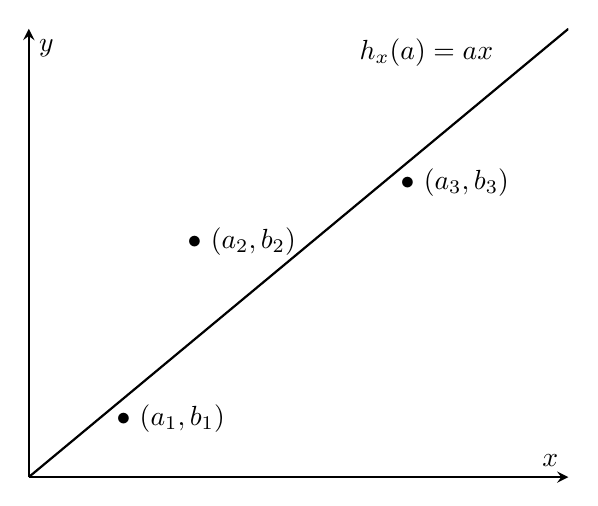
\begin{tikzpicture}
\begin{axis}[ xlabel={$x$}, ylabel={$y$}
,axis lines=middle
, thick
,domain=0:4
,ticks=none
]
\addplot[domain=0:3.8,samples=5000] {x};
\node at (2.8,3.6){$h_x(a)=ax$};
\node at (1,0.5){$\bullet\,\,(a_1,b_1)$};
\node at (1.5, 2){$\bullet\,\,(a_2,b_2)$};
\node at (3,2.5){$\bullet\,\,(a_3,b_3)$};
\end{axis}
\end{tikzpicture}
\end{center}

\note How to get a hyperplane (or line) that does not contain the origin?

Let $n=k+1, a_{i,k+1}=1,\forall i$, then $h_x(a_i)=x_1a_{i1}+\cdots+x_ka_{ik}+x_{k+1}$
\begin{align*}
    f(x)&=\sum_i(a_i^Tx-b_i)^2=(Ax-b)^2=(Ax-b)^T(Ax-b)=||Ax-b||^2_2\\
    &=x^TA^TAx-x^TA^Tb-b^TAx+b^Tb\\
    &=x^T(A^TA)x-(2A^Tb)^Tx+b^Tb
\end{align*}

Thus $f(x)$ is a quadratic function

If $rank(A)=n$, we have seen that $||Ax-b||_2$ is coercive, so it has a global minimizer. 

If $rank(A)=n$ and $A^TA$ is p.d., then $f(x)$ has a global minimizer
\begin{center}$x^*=-\frac{1}{2}(A^TA)^{-1}(-2A^Tb)=(A^TA)^{-1}A^Tb$
\end{center}

\section{Nonlinear Least Squares}

Let $g:\bR^n\to\bR^m$ with $g_i(x)=h_x(a_i)-b$, we have $f(x)=\sum_i\big(g_i(x)\big)^2=g(x)^Tg(x)$

\defn[Jacobian Matrix]
The Jacobian matrix of $g$ is given by 
    $J(x)=\begin{bmatrix}
    \nabla g_1(x)^T\\
    \vdots\\
    \nabla g_m(x)^T
    \end{bmatrix}=\begin{bmatrix}
    &\frac{\partial}{\partial x_1}g_1(x)\,&\,\cdots\,&\frac{\partial}{\partial x_n}g_1(x)\\
    &\vdots\,&\ddots\,& \vdots\\
    &\frac{\partial}{\partial x_1}g_m(x)\,&\,\cdots\,&\frac{\partial}{\partial x_n}g_m(x)\\
    \end{bmatrix}$

\begin{align*}
    \frac{\partial}{\partial x_k}f(x)&=\frac{\partial}{\partial x_k}\sum_i\big(g_i(x)\big)^2\\
    &=\sum_i 2g_i(x)\frac{\partial}{\partial x_k}g_i(x)\\
    &=2 e_k^T J(x)^T g_i(x)
\end{align*}

Thus $\nabla f(x)=2 J(x)^Tg(x)$

\note
If $g_i(x^*)=0$, then $\nabla f(x^*)=0$ and $x^*$ is a global minimizer
\begin{align*}
    \frac{\partial^2}{\partial x_k\partial x_l}g(x)&=\frac{\partial}{\partial x_l}2\big(\sum_i g_i(x)\frac{\partial}{\partial x_k} g_i(x)\big)\\
    &=2\sum_i\big(\frac{\partial}{\partial x_l}g_i(x)\frac{\partial}{\partial x_k}g_i(x)+g_i(x)\frac{\partial^2}{\partial x_k\partial x_l}g_i(x)\big)\\
    \nabla^2 f(x)&=\big(2\sum_i\underbrace{g_i(x)\nabla^2g_i(x)}_{\mbox{not necessary p.d.}}\big)+2\underbrace{J(x)^TJ(x)}_{\mbox{p.s.d}}
\end{align*}

\chapter{Descent Algorithms}

{\bf General Framework}
\begin{align*}
    \mbox{Choose }& x^0\in\bR^n\\
    \mbox{for }& k=0,1,2,\cdots\\
    &\mbox{Choose a search direction }p^k\in\bR^n\\
    &\mbox{Choose a step length }\alpha^k>0\\
    &\mbox{Let }x^{k+1}=x^k+\alpha^2p^k
\end{align*}
\note $\alpha^k$ is not $\alpha$ to the power $k$, same for $p^k,x^k$. Also the objective function $f(x^{k+1})$ should be much smaller than $f(x^k)$ and $x^k$ converges as fast as possible

$\ $

{\bf Steepest Descent} $p^k=-\nabla f(x^k)$

$\ $

\lemma[From Limit to Bound]
Let $\lim_{\epsilon\to 0, \epsilon>0}\frac{\phi(\epsilon h)}{\epsilon}=0$ for any $K>0$, there exists $\epsilon$ small enough such that $|\phi(\epsilon h)|\leq \epsilon K$
\begin{proof}
For any $K>0$, there exists $\gamma>0$ such that $|\frac{\phi(\epsilon h)}{\epsilon}-0|\leq K, \forall 0<\epsilon \gamma$, i.e. 
\begin{align*}
    |\phi(\epsilon h)|\leq \epsilon K, \forall 0<\epsilon <\gamma
\end{align*}
Thus $\epsilon$ sufficiently small is $\epsilon\leq \gamma$
\end{proof}

\thm
Let $f\in C^1\big(B_t(x^k)\big), t>0$ and $\nabla f(x^k)\neq 0$. Consider the optimization problem, for some $0<\epsilon<t, \min\{f(x^k+\epsilon p)\,:\,||p||_2=1\}$. 
Let $p^*$ be a minimizer, then $\lim_{\epsilon\to 0}p^*_{\epsilon}=-\frac{\nabla f(x^k)}{||\nabla f(x^k)||}$
\begin{proof}
Let $x=x^k, p=-\frac{\nabla f(x)}{||\nabla f(x)||_2}$, hence $\nabla f(x)=-p||\nabla f(x)||$

Let $u\in\bR^n$ with $||u||_2=1, u\neq p$, so $||u-p||>\delta>0$, hence
\begin{align*}
    (u-p)^T(u-p)&>\delta^2\\
    u^Tu-2u^Tp+p^Tp&>\delta^2\\
    2-2u^Tp&>\delta^2\\
    u^Tp&<1-\frac{\delta^2}{2}
\end{align*}

{\bf First use Taylor to write $f(x+\epsilon u)$}
\begin{align*}
    f(x+\epsilon u)&=f(x)+\epsilon u^T\nabla f(x)+\phi(\epsilon u),\mbox{ with }\lim_{\epsilon\to 0}\frac{\phi(\epsilon u)}{\epsilon}=0\\
    &=f(x)-\epsilon ||\nabla f(x)||u^Tp+\phi(\epsilon u)\\
    &\geq f(x)-\epsilon ||\nabla f(x)||(1-\frac{\delta^2}{2})+\phi(\epsilon u)
\end{align*}
Now we want to get rid of $\phi(\epsilon u)$.
For $\epsilon$ small enough, by Lemma 7.0.1, we have
\begin{align*}
    |\phi(\epsilon u)|&\leq \epsilon(||\nabla f(x)||\frac{\delta^2}{4})\\
    \phi(\epsilon u)&\geq -\epsilon||\nabla f(x)||\frac{\delta^2}{4}
\end{align*}

Hence we have a lower bound
\begin{align*}
    f(x+\epsilon u)&\geq f(x)-\epsilon ||\nabla f(x)||(1-\frac{\delta^2}{2})-\epsilon||\nabla f(x)||\frac{\delta^2}{4}\\
    &=f(x)-\epsilon||\nabla f(x)||+\epsilon \frac{\delta^2}{4}||\nabla f(x)||
\end{align*}

{\bf Then use Taylor to write $f(x+\epsilon p)$}
\begin{align*}
    f(x+\epsilon p)&=f(x)+\epsilon p^T\nabla f(x)+\phi(\epsilon p),\mbox{ with }\lim_{\epsilon\to 0}\frac{\phi(\epsilon p)}{\epsilon}=0\\
    &=f(x)-\epsilon ||\nabla f(x)||p^Tp+\phi(\epsilon p)\\
    &=f(x)-\epsilon ||\nabla f(x)||+\phi(\epsilon p)
\end{align*}

Again, for $\epsilon$ small enough, combined with the lower bound, we choose our magic upper bound
\begin{align*}
    |\phi(\epsilon p)|&\leq \epsilon \frac{\delta^2}{5}||\nabla f(x)||\\
    \phi(\epsilon p)&\leq \epsilon \frac{\delta^2}{5}||\nabla f(x)||
\end{align*}

Hence we have a upper bound
\begin{align*}
    f(x+\epsilon p)\leq f(x)-\epsilon ||\nabla f(x)||+\epsilon \frac{\delta^2}{5}||\nabla f(x)||
\end{align*}

{\bf Using two bounds, we have}
\begin{align*}
    f(x+\epsilon p)\leq f(x)-\epsilon ||\nabla f(x)||+\epsilon \frac{\delta^2}{5}||\nabla f(x)||\leq f(x)-\epsilon||\nabla f(x)||+\epsilon \frac{\delta^2}{4}||\nabla f(x)||\leq f(x+\epsilon u)
\end{align*}

Therefore $f(x+\epsilon p)$ is the minimizer
\end{proof}

\defn[Descent Direction]
$p^k$ is a descent direction if $f(x^k+\epsilon p^k)<f(x^k)$, for all $\epsilon $ small enough

\thm
Let $x^k$ be such that $\nabla f(x^k)\neq 0$, if $(p^k)^T\nabla f(x^k)<0$, then $p^k$ is a descent direction
\begin{proof}
Let $p=p^k$, WLOG, $||p||=1$, by Taylor, have
\begin{align*}
    f(x^k+\epsilon p)=f(x)+\epsilon p^T\nabla f(x^k)+\phi(\epsilon p), \mbox{ with }\lim_{\epsilon \to 0} \frac{\phi(\epsilon p)}{\epsilon }=0
\end{align*}

For $\epsilon $ small enough, $|\phi(\epsilon p)|\leq \epsilon |\frac{1}{2}p^T\nabla f(x^k)|=-\epsilon \frac{1}{2}p^T\nabla f(x^k)$

Hence we have
\begin{align*}
    f(x^k+\epsilon p)\leq f(x^k)+\frac{1}{2}\epsilon p^T\nabla f(x)<f(x^k)
\end{align*}
\end{proof}

\section{Line Search}
{\bf Once $p^k$ is chosen, determine $\alpha^k$ such that $x^{k+1}=x^k+\alpha^k+p^k$}

$\bullet$ Exact Line Search : $\alpha^k=argmin_{\alpha\geq 0}\{f(x^k+\alpha p^k)\}$

We define $\psi(\alpha)=f(x^k+\alpha p^k)$

\note $\psi(0)=f(x^k)$ and once $\alpha^k$ is chosen, $\psi(\alpha^k)=f(x^{k+1})$

$\psi'(\alpha)=\frac{d}{d\alpha}\psi(\alpha)=\nabla f(x^k+\alpha p^k)^Tp^k$ (directional derivative)

$\psi'(0)=\nabla f(x^k)^Tp^k<0$ since we assume $p^k$ is a descent direction

\begin{figure}[ht!]
	\centering
	\includegraphics[width=14cm, height=10cm]{linesearch.jpg}
\end{figure}

{\bf Sufficient Decrease Condition :} Fix $0<\sigma<\frac{1}{2}$, $\alpha$ must satisfy that :
\begin{align*}
    \psi(\alpha)\leq \psi(0)+\sigma \alpha\psi'(0)
\end{align*}

{\bf Curvature Condition (Scveral Variants}
\begin{align*}
    \psi(2\cdot \alpha)>\psi(0)+\sigma 2\alpha \psi'(0)
\end{align*}

$\ $

{\bf Armijo ("backtrack") Inexact Linea Search}

Let $\alpha :=1$

If $\alpha$ fails sufficient decrease

\hspace{1cm} While $\alpha$ fails sufficient decrease

\hspace{2cm} $\alpha :=\alpha /2$

Else $\alpha$ fails curvature condition

\hspace{1cm} While $\alpha$ fails curvature condition

\hspace{2cm} $\alpha :=\alpha/2$

\thm
Let $f\in C^1, \nabla f(x^k)\neq 0$ and let $p^k$ be a descent direction, then

Either the Armijo Algorithm terminates and $\alpha $ satisfies both conditions

Or $\alpha\to +\infty$ and $f$ is unbounded below $(f(x^k)\to -\infty)$

\begin{proof}
$\bullet$ If the first loop terminates, $\alpha$ satisfies sufficient decrease and $2\alpha$ fails it, i.e. $\alpha$ satisfies curvature condition

We need to show that the first loop terminates:
\begin{align*}
    \psi(\alpha)=\psi(0)+\alpha\cdot\psi'(0)+\phi(\alpha)
\end{align*}

For $\alpha$ sufficient small, by Lemma 7.0.1, have 
\begin{align*}
    |\phi(\alpha)|&\leq \alpha|\frac{1}{2}\psi'(0)|\\
    \phi(\alpha)&\leq -\alpha\frac{1}{2}\psi'(0)
\end{align*}

Thus $\psi(\alpha)\leq \psi(0)+\frac{1}{2}\psi'(0)\cdot\alpha$

$\bullet$ If the second loop terminates, $\alpha$ satisfies curvature condition, $\frac{\alpha}{2}$ fails it, i.e. $\alpha$ satisfies sufficient decrease

$\bullet$ If the second loop does not terminate, 
\begin{align*}
    \psi(2^j)\leq \psi(0)+2^j\sigma \underbrace{\psi'(0)}_{<0}, \forall j\in\bZ^+
\end{align*}

Thus $\psi(2^j)\to-\infty$ for $j\to +\infty$

$\bullet$ If we did not go in either loop, $\alpha=1$ satisfies both conditions
\end{proof}

\defn[Lipschitz Continuous]
A function $f:\bR^n\to \bR$ is Lipschitz continuous with constant $L$ if $|f(y)-f(x)|\leq L\cdot\,||y-x||, \forall x,y\in\bR^n$

\note Lipschitz continuous implies $C^0$ continuous, but the converse is not true

\thm
Let $f\in C^1\big(B_{\delta}(0)\big),\,\, f$ is Lipschitz continuous with constant $L$ on $B_{\delta}(0)$ if and only if $||\nabla f(x)||\leq L, \forall x\in B_{\delta}(0)$

\thm[Zoutendijk's Thm]
Let $f:\bR^n\to\bR$ with $f\in C^1(\bR^n)$. If

(1) $\nabla f$ is Lipschitz continuous

(2) $\forall k$, $p^k$ is a descent direction with $\nabla f(x^k)^Tp^k\leq -\mu ||\nabla f(x^k)||_2\cdot||p^k||_2$ for some $0<\mu\leq 1$. This means if $\mu=1$, then $p^k$ would be the steepest direction (think of vector dot product, $\mu$ would be a cosine of an angle)

(3) $\forall k$, $\alpha^k$ satisfies both decrease and curvature condition

Then either (a) $\lim_{k\to \infty} f(x^k)=-\infty$, or (b) $\lim_{k\to \infty} \nabla f(x^k)=0$
\begin{proof}
We will prove there is no other situation (c), i.e. if (b) does not happen, then (a) does

Note that (b) $\lim_{k\to \infty} \nabla f(x^k)=0$ can be stated in the following way
\begin{align*}
    \forall \epsilon >0, \,\exists\,K\geq 0\,:\,\forall k\geq K, \,||\nabla f(x^k)||<\epsilon
\end{align*}

If instead (b) does not happen, i.e. $\lim_{k\to \infty} \nabla f(x^k)$ does not exists or not equal to 0, then
\begin{align}
    \exists \epsilon >0\,,\,\forall \,K>0, \,,\,\exists\,k\geq K\,:\,||\nabla f(x^k)||\geq \epsilon
\end{align}

In the rest of the proof, we will show that (7.1) implies $f(x^{k+1})\leq f(x^k)-\delta$ for some constant $\delta>0$, thus $f(x^k)\to-\infty$

We need to find a upper bound of $\psi(\alpha^k)$, note that $\psi'(0)<0$, we must find a lower bound of $\alpha^k$

Now consider for some $0<\sigma<\frac{1}{2}$, the curvature condition gives:
\begin{align*}
    \psi(2\alpha^k)>\psi(0)+2\alpha^k\sigma\psi'(0)
\end{align*}

And the mean value thm
\begin{align*}
    \exists\,0\leq \gamma\leq 2\alpha^k\,\psi(2\alpha^k)=\psi(0)+2\alpha^k\psi'(\gamma)
\end{align*}

Together we have
\begin{align}
    \psi'(\gamma)&>\sigma \psi'(0)\nonumber \\
    \nabla f(x^k+\gamma p^k)^Tp^k&>\sigma \nabla f(x^k)^Tp^k
\end{align}

Then consider Lipschitz gives
\begin{align*}
    ||\nabla f(x^k+\gamma p^k)-\nabla f(x^k)||\leq L\cdot\gamma||p^k||
\end{align*}

And the CS inequality gives
\begin{align}
    [\nabla f(x^k+\gamma p^k)-\nabla f(x^k)]^Tp^k&\leq ||\nabla f(x^k+\gamma p^k)-\nabla f(x^k)||\cdot||p^k||\nonumber\\
    &\leq L\cdot\gamma||p^k||^2\nonumber\\
    \nabla f(x^k+\gamma p^k)^Tp^k&\leq \nabla f(x^k)^Tp^k+L\cdot\gamma ||p^k||^2
\end{align}

Combined (7.2) and (7.3) together, have
\begin{align*}
    \nabla f(x^k)^Tp^k+L\cdot\gamma ||p^k||^2&>\sigma \nabla f(x^k)^Tp^k\\
    L\cdot\gamma ||p^k||^2&>(\sigma-1) \nabla f(x^k)^Tp^k\\
    L\cdot\gamma ||p^k||^2&>(\sigma-1) \psi'(0)\\
    \gamma&>\frac{(1-\sigma)(-\psi'(0))}{L\cdot||p^k||^2}
\end{align*}

Recall that $0\leq \gamma\leq 2\alpha^k$, thus $\alpha^k\geq \gamma/2$, hence {\bf finally we get an lower bound for $\alpha^k$}
\begin{align*}
    \alpha^k>\frac{(1-\sigma)(-\psi'(0))}{2L\cdot||p^k||^2}
\end{align*}

Now we show the sufficient decrease
\begin{align*}
    \psi(\alpha^k)&\leq \psi(0)+\sigma \alpha^k\psi'(0)\\
    &\leq \psi(0)+\sigma\frac{(1-\sigma)(-\psi'(0))}{2L\cdot||p^k||^2}\psi'(0)\,\,\mbox{ note }\psi'(0)<0\\
    &=\psi(0)-\frac{\sigma(1-\sigma)}{2L}\cdot\big(\frac{\psi'(0)}{||p^k||^2})^2
\end{align*}

By hypothesis
\begin{align*}
    \big(\psi'(0)\big)^2=\big(\nabla f(x^k)^Tp^k\big)^2\geq \mu^2\cdot||
    \nabla f(x^k)||^2\cdot||p^k||^2
\end{align*}

Hence we have
\begin{align*}
    \psi(\alpha^k)\leq \psi(0)-\frac{\sigma(1-\sigma)}{2L}\cdot\mu^2\cdot||\nabla f(x^k)||^2
\end{align*}

By (7.1), $||\nabla f(x^k)||\geq \epsilon$, so
\begin{align*}
    \psi(\alpha^k)&\leq \psi(0)-\frac{\sigma(1-\sigma)\mu^2\epsilon^2}{2L}\\
    f(x^k+\alpha^kp^k)&\leq f(x^k)-\frac{\sigma(1-\sigma)\mu^2\epsilon^2}{2L}
\end{align*}
\end{proof}

$\ $

$\bullet$ We now have a complete algorithm:

\hspace{0.5cm} Start at an arbitrary $x^0\in\bR^n$

\hspace{0.5cm} For $k=1,2,\cdots$

\hspace{1cm} Choose $p^k$ such that $\nabla f(x^k)^Tp^k\leq -\mu\cdot||\nabla f(x^k)||\cdot||p^k||$, for some $0<\mu\leq 1$

\hspace{2cm} for example $p^k:=-\nabla f(x^k)$, the steepest descent 

\hspace{1cm} Choose $\alpha^k$ with Armijo inexact line search

\hspace{1cm} Let $x^{k+1}:=x^k+\alpha^kp^k$

\hspace{1cm} If ($f(x^{k+1}<-M$) or ($||\nabla f(x^{k+1})||\,\leq \epsilon$)

\hspace{2cm} STOP

\section{Convergence of Descent Algorithms}

\defn[Converge Degree]
A sequence $s^0,s^1,\cdots$ converges with degree $d$ to 0 if $|s^{k+1}|\leq C\cdot |s^k|^d$. Convergence is said to be linear if $d=1$ and quadratic if $d=2$

\defn[Strongly Convex]
A function $f\in C^1(\bR^n)$ is strongly convex if $\big(\nabla f(y)-\nabla f(x)\big)^T(y-x)\geq l\cdot ||y-x||^2,\forall x,y\in\bR^n$ for some $l>0$

\lemma
If $f$ is strongly convex, then $||\nabla f(y)-\nabla f(x)||^2\geq l\cdot |f(y)-f(x)|,\forall x,ty\in\bR^n$

%eigenvalue >= l??

\lemma[Assignment 1 Q2]
Let $f\in C^2(\bR^n)$, $f$ is strongly convex if and only if $\big(\nabla^2f(x)-l\cdot I\big)$ is p.s.d. for all $x\in\bR^n$

\lemma 
Any strongly convex function is strictly convex

\thm
Assume the same condition as Zoutendijk's Thm, if in addition, $f$ is strongly convex, then $f(x^k)$ converges linearly to a local( global ) minimizer $f(x^*)$
\proof
From the previous proof we have
\begin{align*}
f(^{k+1})&\leq f(x^k)-\frac{\sigma(1-\sigma)\mu^2}{2L}||\nabla f(x^k)||^2\\
f(^{k+1})-f(x^*)&\leq f(x^k)-f(x^*)-\frac{\sigma(1-\sigma)\mu^2}{2L}||\nabla f(x^k)||^2
\end{align*}
By Lemma 7.2.1, $||\nabla f(x^k)-\overline{\nabla f(x^*)}_{0}||^2\geq l\cdot |f(x^k)-f(x^*)|$

I.e. we get an lower bound $||\nabla f(x^k)||^2\geq l\cdot\big(f(x^k)-f(x^*)\big)$, hence
\begin{align*}
    f(^{k+1})-f(x^*)&\leq f(x^k)-f(x^*)-\frac{\sigma(1-\sigma)\mu^2}{2L}||\cdot l\cdot\big(f(x^k)-f(x^*)\big)\\
    &\leq \big(f(x^k)-f(x^*)\big)(1-\overline{\frac{\sigma(1-\sigma)\mu^2l}{2L}}_{>0,<1}
\end{align*}

Thus the sequence $\big(f(x^k)-f(x^*)\big)$ converges linearly to 0

\thm
For a strongly convex quadratic function, the steepest descent method with exact line search has $||x^k-x^*||$ converges linearly to 0. Also this bound is tight, i.e. cannot converge with $d>1$

Thm 7.2.1 shows that in many cases, the sequence converges linearly and Thm 7.2.2 shows that not many can converge over linealy, this leads to the next section

\section{Newton Step}
Consider a quadratic approximation of $f$ at $x^k$ : 
\begin{align*}
    f(x^k+h)\approx q(h)=f(x^k)+h^T\nabla f(x^k)+\frac{1}{2}h^T\nabla^2 f(x)h
\end{align*}

If( and only if ) $\nabla f^2(x^k)$ is p.d., $q(h)$ has a unique minimizer $h=-[\nabla^2f(x^k)]^{-1}\nabla f(x^k)$

The newton step is given by taking $p^k=-[\nabla^2f(x^k)]^{-1}\nabla f(x^k)$, note clearly it only works if the $\nabla^2(f^k)$ is p.d.

\defn[Linearly \& Quadratic Convergence]
A sequence $s^0,s^1,\cdots$ converges linearly to zero if $|s^{k+1}\leq C\cdot |s^k|$ for some $0<C<1$, the sequence converges quadratically if $|s^{k+1}|\leq C\cdot |s^k|^2$ for some $C>0$

\note Newton's Method : $x^{k+1}=x^k-\nabla^2 f(x^k)^{-1}\nabla f(x^k)$

\lemma
Let $F:\bR^n\to\bR^{m\times m}$ be continuous over $B_r(x_0)$ for some $x_0\in\bR^n$ such that $F(x_0)$ is nonsingular. Then there exists $R>0$ such that $F(x)$ is invertible for all $x\in B_R(x_0)$ and $F(x)^{-1}$ is continuous over $B_R(x_0)$
\proof
Given any matrix $A\in\bR^{m\times m}$, $det(A)$ is a polynomial in all entries of $A$

Since $det\big(F(x_0)\big)\neq 0$, then there exists $R>0$ such that $det\big(F(x)\big)\neq 0$ for all $x\in B_R(x_0)$

Still given $A\in \bR^{m\times m},\,(A^{-1})_{ij}=\frac{P}{det(A)}$ where $P$ is a polynomial in entries of $A$

Thus $\big(F(x)^{-1})$ is a polynomial in $F(x)$ divided by another nonzero polynomial, hence it is continuous

\thm
Let $f:\bR^n\to\bR$ be such that $f\in C^2(\big(B_r(x^*)\big)$, if 

(1) $\nabla^2 f$ is Lipschitz continuous over $B_r(x^*)$, i.e.
\begin{align*}
    ||\nabla^2 f(y)-\nabla^2 f(x)||_2\leq L\cdot ||y-x||_2
\end{align*}
(2) $\nabla f(x^*)=0$ and $\nabla^2 f(x^*)$ is p.d. (2nd order sufficient conditions for local optimality)

(3) $\nabla^2 f(x)^{-1}||\leq 2||\nabla^2f(x^*)^{-1}||$ for all $x\in B_r(x^*)$ (By lemma, there exists $r$ sufficiently small such that this is satisfied)

(4) $r\leq \frac{1}{2L||\nabla^2f(x^*)^{-1}||}$

Then Newton's Method converges quadratically to $x^*$ if $x^0\in B_r(x^*)$
\proof
Assume for induction that $x^k\in B_r(x^*)$, we will show that $x^{k+1}\in B_r(x^*)$
\begin{align*}
    x^{k+1}-x^*&=x^k-\nabla^2f(x^k)^{-1}\nabla f(x^k)-x^*\\
    &=\nabla^2 f(x^k)^{-1}\cdot\big(\nabla^2f(x^k)(x^k-x^*)-(\nabla f(x^k)-\overline{\nabla f(x^*)}_{=0}\big)\\
    &=\nabla^2 f(x^k)^{-1}\cdot \big(\int_0^1\underbrace{\nabla^2 f(x^k)(x^k-x^*)dt}_{\mbox{does not vary with }t}-\int_0^1\underbrace{\nabla^2 f(x^*+t(x^k-x^*))(x^k-x^*)dt}_{\begin{subarray}{l}\text{directional derivative of $\nabla f$}\\
    \text{in direction $(x^k-x^*)$}\\
    \text{integrated from $x^*$ to $x^k$}\end{subarray}}\\
    &=\underbrace{\nabla^2 f(x^k)^{-1}}_{(a)}\cdot\underbrace{\int_0^1\big(\nabla^2f(x^k)-\nabla^2f(x^*+t(x^k-x^*))\big)(x^k-x^*)dt}_{(b)}
\end{align*}
\begin{align*}
(a)\,:\,&||\nabla^2 f(x^k)^{-1}||\leq 2\cdot ||\nabla^2 f(x^*)^{-1}||\mbox{ by (3)}\\
(b)\,:\,&\,\,||\int_0^1\big(\nabla^2f(x^k)-\nabla^2f(x^*+t(x^k-x^*))\big)(x^k-x^*)dt||\\&\leq \int_0^1||(\nabla^2f(x^k)-\nabla^2f(x^*+t(x^k-x^*))||\cdot ||x^k-x^*||dt\\
&\leq \int_0^1L\cdot ||x^k-x^*-t(x^k-x^*)||\cdot||x^k-x^*||dt\\
&\leq L\cdot \int_0^1||(x^k-x^*)(1-t)||\cdot ||x^k-x^*||dt\\
&=L\cdot ||x^k-x^*||^2\int_0^1(1-t)dt\\
&=\frac{L\cdot ||x^k-x^*||^2}{2}
\end{align*}

Therefore have
\begin{align*}
    ||x^{k+1}-x^*||\leq 2\cdot ||\nabla^2 f(x^*)^{-1}||\cdot \frac{L\cdot ||x^k-x^*||^2}{2}
\end{align*}

By induction, we have $||x^k-x^*||\leq r$ and by (4) $r\leq \frac{1}{2L||\nabla^2f(x^*)^{-1}||}$, hence have
\begin{align*}
    ||x^{k+1}-x^*||\leq \frac{1}{2r}||x^k-x^*||^2
\end{align*}

So the convergence (if any) is quadratic

And since $||x^k-x^*||\leq r$, we have $||x^{k+1}-x^*||\leq \frac{1}{2}||x^k-x^*||$

Therefore we have the convergence

\chapter{Trust Region Methods}

{\bf Algorithm}

Choose $x^0$ arbitrarily

Let $\delta^0=1$

For $k=0,1,\cdots$

\hspace{1cm} Let $q(x)$ be a quadratic approximation of $f$ that is accurate around $x^k$

\hspace{1cm} $x^{TEST}:=argmin\{q(x):||x-x^k|\leq \delta^k\}$

\hspace{1cm} $\rho:=\frac{f(x^k)-f(x^{TEST})}{q(x^k)-q(x^{TEST})}\,\,$ // The ratio of decrease

\hspace{2cm} If $\rho\geq 1/8$

\hspace{3cm} $x^{k+1}=x^{TEST}$

\hspace{2cm} Else $x^{k+1}=x^k$

\hspace{2cm} If $\rho\leq 1/4$

\hspace{3cm} $\delta^{k+1}=\delta^k/2$

\hspace{2cm} Else if $\rho\geq 3/4$ and $||x^{TEST}-x^k||=\delta^k$

\hspace{3cm} $\delta^{k+1}=2\cdot \delta^k$

\hspace{2cm} Else $\delta^{k+1}=\delta^k$

\begin{figure}[ht!]
	\centering
	\includegraphics[width=14cm, height=10cm]{trustregionalg.jpg}
\end{figure}

\note 
$\bullet$ There are other possible choices, but we consider 
\begin{align*}
    q(x)=f(x^k)+(x-x^k)^T\nabla f(x^k)+\frac{1}{2}(x-x^k)^T\nabla^2f(x^k)(x-x^k)
\end{align*}
$\bullet$ $\rho$ is the ratio $\frac{\mbox{decrease in }f}{\mbox{decrease in }q}$ from $x^k$ to $x^{TEST}$. The decrease in $q$ is guaranteed $\geq 0$ since $q(x^k)$ is considered in the agrmin set.

$\bullet$ If $x^{TEST}=x^k$, then the 2nd order sufficient conditions are satisfied. $\rightarrow$ STOP

$\bullet$ $\delta^k$ is the {\bf Trust Region Radius}. We consider $q$ is a "good" approximation of $f$ in $B_{\delta^k}(x^k)$. If $\rho$ is small, the approximation is bad, and we decrease $\delta^k$

\thm
Let $f\in C^2(\bR^n)$ and assume that $\nabla^2f$ is Lipschitz continuous in a ball that contains the level set of $x^0$. Then for the trust region method

(1) Either $x^k\to-\infty$ or $\nabla f(x^k)\to 0$ (similar as descent method)

(2) If $x^k\to x^*$, then $x^*$ satisfies 1st and 2nd order necessary condition for local optimality

(3) If $x^k\to x^*$ and $x^*$ satisfies the 1st and 2nd sufficient conditions for local optimality, then for $k$ large enough, $||x^{TEST}-x^k||\leq \delta^k$, the step is {\bf Newton's Step}, so the convergence is quadratic.

\section{The Trust Region Subproblem (TRS)}
\begin{align*}
    argmin \{\overbrace{f(x^k)}^{constant}+(x-x^k)^T\nabla f(x^k)+\frac{1}{2}(x-x^k)^T\nabla^2f(x^k)(x-x^k)\,:\,||x-x^k||\leq 1\}
\end{align*}

For simplicity, let $\tilde{x}=\frac{x-x^k}{\delta^k}$, we get
\begin{align*}
    &agrmin\{\big(\delta^k\nabla f(x^k)\big)^T\cdot \tilde{x}+\tilde{x}^T\big((\delta^k)^2\frac{1}{2}\nabla^2 f(x^k)\big)\tilde{x}\,:\,||\tilde{x}||\leq 1\}\\
    =&argmin\{x^TAx+b^Tx:||x||\leq 1\}\,\mbox{where }A=\frac{(\delta^k)^2}{2}\nabla^2f(x^k),b=\delta^k\nabla f(x^k)
\end{align*}


How do we solve (TRS)?
\begin{align*}
    &min\,\,\,\,x^TAx+b^Tx\\
    &s.t.\,\,\,\,\,\,\,\,\,||x|\leq 1
\end{align*}

If $A$ is p.d., then we can compute $\hat{x}=-\frac{1}{2}A^{-1}b$

{\bf CASE 1} $A$ is p.d. and $||\hat{x}||=||-\frac{1}{2}A^{-1}b||\leq 1$. Then $\hat{x}$ is optimal for (TRS)

{\bf CASE 2} $A$ is not p.d. or $||\hat{x}||>1$. Let $\hat{x}(\lambda)=-\frac{1}{2}(A+\lambda I)^{-1}b$

\note
$\bullet$ $(A+\lambda I)$ shifts all the eigenvalue, so at some point, all the eigenvalue would be positive thus the inverse $(A+\lambda I)^{-1}$ is well-defined.

$\bullet$ Let $\lambda_1\leq \cdots\leq \lambda_n$ be the eigenvalues of $A$, $\hat{x}$ is defined for all $\lambda>-\lambda_1$

$\bullet$ $\hat{x}(0)$ would be optimal in {\bf CASE 1}

$\bullet$ $\hat{x}(\lambda)$ would be a global minimizer for $x^T(A+\lambda I)x+b^Tx$

\thm
$||\hat{x}(\lambda)||$ is a decreasing function of $\lambda$ over $(-\lambda_1,-\infty)$. Moreover $\lim_{\lambda\to\infty}||\hat{x}(\lambda)||=0$
\proof
Let $A=QDQ^T$ where $Q$ is orthogonal and $D=diag(\lambda_1,\cdots,\lambda_n)$

Observe that for all $z\in\bR^n$, $||Qz||=||z||$ since $||Qz||^2=(Qz)^T(Qz)=z^TQ^TQz=z^Tz=||z||^2$ or intuitively $Qz$ is a rotation of $z$ as $Q$ is orthogonal. Thus
\begin{align*}
    \hat{x}(\lambda)&=-\frac{1}{2}(QDQ^T+\lambda I)^{-1}b\\
    &=-\frac{1}{2}(QDQ^T+\lambda QIQ^T)^{-1}b\\
    &=-\frac{1}{2}[Q(D+\lambda I)Q^T]^{-1}b\\
    &=-\frac{1}{2}Q^{T^{-1}}(D+\lambda I)^{-1}Q^{-1}b\\
    &=-\frac{1}{2}Q(D+\lambda I)^{-1}Q^Tb\\
    ||\hat{x}(\lambda)||&=\frac{1}{2}||Q(D+\lambda I)^{-1}Q^Tb||\\
    &=\frac{1}{2}||(D+\lambda I)^{-1}\underbrace{Q^Tb}_{c}||\,\,\mbox{ by }||Qz||=||z||\\
    &=\frac{1}{2}||(D+\lambda I)^{-1}c||\\
    &=\frac{1}{2}||(\begin{bmatrix}
    \lambda_1\,&\,0\,\cdots\,0\\
    0\,&\lambda_2\,&\,\cdots\,0\\
    \vdots\,&\,\vdots\,&\,\ddots\,&\,\vdots\\
    0\,&\,0\,&\,\cdots\,\lambda_n
    \end{bmatrix}+\lambda I)^{-1}\cdot c||\\
    &=\frac{1}{2}||\begin{bmatrix}
    \frac{1}{\lambda_1+\lambda}\,&\,0\,\cdots\,0\\
    0\,&\frac{1}{\lambda_2+\lambda}\,&\,\cdots\,0\\
    \vdots\,&\,\vdots\,&\,\ddots\,&\,\vdots\\
    0\,&\,0\,&\,\cdots\,\frac{1}{\lambda_n+\lambda}
    \end{bmatrix}\cdot c||\\
    &=\frac{1}{2}||\begin{bmatrix}
     \frac{c_1}{\lambda_1+\lambda}\\
      \frac{c_2}{\lambda_2+\lambda}\\
      \vdots\\
       \frac{c_n}{\lambda_n+\lambda}
    \end{bmatrix}||\\
    &=\frac{1}{2}\sqrt{\sum_i\underbrace{(\frac{1}{\lambda_i+\lambda})^2}_{decreasing\,\,for\,\,\lambda>-\lambda_i}\cdot\underbrace{c_i^2}_{constant\,\,\geq 0}}\\
    \lim_{\lambda\to\infty}||\hat{x}(\lambda)||&=0
\end{align*}

{\bf CASE 2a : }$c_1\neq 0, \lambda_1\neq 0$
\note $c_1=(Q^Tb)_1=v_1^Tb=v^T_1\nabla f(x^k)\delta^k$, where $v_1$ is the eigenvector of $\nabla^2f(x^k)$ corresponding to $\lambda_1$ ($||v_1||=1$), so $c_1\neq 0$ means $\nabla f(x^k)$ is not orthogonal to $v_1$

In this case, $\lim_{\lambda\to\-\lambda_1}||\hat{x}(\lambda)||=+\infty$

Then $\exists\,\lambda^*$ such that $||\hat{x}(\lambda^*)||=1$

\begin{figure}[ht!]
	\centering
	\includegraphics[width=10cm, height=5cm]{lambdafunction.jpg}
\end{figure}

\lemma
If $\hat{x}$ is a global minimizer for (TRS) in {\bf CASE 2a}, then $||\hat{x}||=1$
\proof
If $||\hat{x}||<1$, then $\exists\,B_{\delta}(\hat{x})\subseteq B_1(0)$

Since $\hat{x}$ is a global minimizer, it is also a local minimizer for $x^TAx+b^Tx$

If $\lambda_1<0$, $A$ is not p.s.d. and $x^TAx+b^Tx$ has no local minimizers. $\lambda_1=0$ excluded by hypothesis of {\bf CASE 2a}

If $\lambda_1>0$, $A$ is p.d. and $x^TAx+b^Tx$ has a unique local (and global) minimizer, but by {\bf CASE 2a} hypothesis, $||\hat{x}||>1$

$\ $

\thm
$\hat{x}(\lambda^*)$ is a global minimizer for (TRS) in {\bf CASE 2a}
\proof
Recall that $\hat{x}(\lambda^*)$ is a global minimizer for $x^T(A+\lambda^*I)x+b^Tx$

If we restrict to $||x||=1$, and we have $||\hat{x}(\lambda^*)||=1$
\begin{align*}
    \hat{x}(\lambda^*)&=argmin\{x^T(A+\lambda^*I)x+b^Tx\,:\,||x||=1\}\\
    &=argmin\{x^TAx+\lambda^*\underbrace{x^Tx}_{||x||^2=1}+b^Tx\,:\,||x||=1\}\\
    &=argmin\{x^TAx+b^Tx+\underbrace{\lambda^*}_{constant}\,:\,||x||=1\}\\
    &=argmin\{x^TAx+b^Tx\,:\,||x||=1\}\\
\end{align*}

By Lemma 8.1.1, $\hat{x}(\lambda^*)=argmin\{x^TAx+b^Tx\,:\,||x||\leq 1\}$

$\ $

{\bf CASE 2b : }either $c_1=0$ or $\lambda_1=0$

\thm
A global minimizer for (TRS) in {\bf CASE 2b} is given by 
\begin{align*}
    \hat{x}=\sum_{i:\lambda_i\neq\lambda_1}\frac{v^T_ib}{\lambda_i-\lambda_1}+\tau v_1
\end{align*}

where $v_i$ is the eigenvector of $A$ corresponding to $\lambda_1,\,||v_i||=1$ and $\tau$ is chosen such that $||\hat{x}||=1$
\proof Nocedal-Weight page 84 "the hard case"

\chapter{Optimality Conditions For Constrained Optimization}

\section{KKT Points}

\defn[Local Minimizer for Constrained OPT \& Feasible Improving Direction]
Consider 
\begin{align*}
    min\,\,&\,f(x)\\
    s.t.\,\,&\,x\in G\subseteq \bR^n
\end{align*}
the point $\hat{x}$ is a local minimizer if $\hat{x}\in G$ and there exists $\epsilon>0$ such that for all $x\in B_{\epsilon}(\hat{x})\cap G$, we must have $f(x)\geq f(\hat{x})$

\note
$\bullet$ The above definition does not require $\big(B_{\epsilon}(\hat{x})\cap G\big)\backslash\{\hat{x}\}\neq \emptyset$, i.e. $\hat{x}$ could be the only point, in which case it is the local minimizer

$\bullet$ Equivalently, $\not\exists\,d\in B_{\epsilon}(0)\,:\,\hat{x}+d\in G$ and $f(\hat{x}+d)<f(\hat{x})$. Such a $d$ would be called a feasible improving direction (or step)

$\ $

Informally, consider 
\begin{align*}
    min\,\,&\,f(x)\\
    s.t.\,\,&\,h(x)=0
\end{align*}
Let $\bar{x}\in\bR^n$ such that $h(\bar{x})=0$. Is there any improving direction $d$ at $\bar{x}$?

If $d$ is small, $h(\bar{x}+d)\approx h(\bar{x})+d^T\nabla h(\bar{x})=d^T\nabla h(\bar{x})$

$\bullet$ $d$ "feasible" : we want $d^T\nabla h(\bar{x})=0$

$\bullet$ $d$ "improving" : we want $d^T\nabla f(\bar{x})<0$

Take an arbitrary such vector $d\perp \nabla h(\bar{x})$.

\hspace{1cm} If $d^T\nabla f(\bar{x})<0$, then we are done

\hspace{1cm} If $d^T\nabla f(\bar{x})>0$, we can take $(-d)$ : have $(-d)^T\nabla h(\bar{x})=0$ and $(-d)^T\nabla f(\bar{x})<0$

\hspace{1cm} If $d^T\nabla f(\bar{x})=0$, we need another direction $d$

When are there {\bf no} feasible improving directions?

When, for all $d\in\bR^n$ such that $d^T\nabla h(\bar{x})=0$, we have $d^T\nabla f(\bar{x})=0$

When all directions orthogonal to $\nabla h(\bar{x})$ are also orthogonal to $\nabla f(\bar{x})$

I.e. when $\nabla h(\bar{x})$ is parallel to $\nabla f(\bar{x})$

Such $\bar{x}$ is called {\bf Karush-Kuhn-Tucker (KKT) Point}

$\ $

\eg
\begin{align*}
    min\,\,&\,x_1+x_2\\
    s.t.\,\,&\,x_1^2+x_2^2-2=0
\end{align*}

where $h$ is a convex function, and the feasible region is the circle of radius $\sqrt{2}$ (just the boundary not include the inside part), which is not convex as there is hole in it.

How can we change $h$ such that the feasible region $h(x)=0$ is also convex? We must need $h$ is a linear function

Note that we want $h(x)=0$ instead of $h(x)\leq 0$, so the thm about convex function and convex set does not work here.

$\nabla f(x)=\begin{bmatrix}
1\\1
\end{bmatrix}$, $\nabla h(x)=\begin{bmatrix}
2x_1\\2x_2
\end{bmatrix}$, KKT points : $\begin{bmatrix}
1\\1
\end{bmatrix}$ and $\begin{bmatrix}
-1\\-1
\end{bmatrix}$ such that $x_1=x_2$

$\ $

Informally, consider \begin{align*}
    min\,\,&\,f(x)\\
    s.t.\,\,&\,g(x)\leq 0
\end{align*} Let $\bar{x}$ be such that $g(\bar{x})\leq 0$

{\bf CASE 1 :} $g(\bar{x})<0$

\hspace{1cm} For all $||d||$ sufficiently small (thus in the feasible region), $g(\bar{x}+d)<0$

\hspace{1cm} We want $d^T\nabla f(\bar{x})<0$, which exists iff $\nabla f(\bar{x})\neq 0$

{\bf CASE 2 :} $g(\bar{x})=0$

\hspace{1cm} $d$ "feasible" : $g(\bar{x}+d)\approx g(\bar{x})+d^T\nabla g(\bar{x})=d^T\nabla g(\bar{x})$, so want $d^T\nabla g(\bar{x})\leq 0$

\hspace{1cm} $d$ "improving" : $d^T\nabla g(\bar{x})<0$

$\ $

When are there {\bf no} feasible improving directions?

{\bf CASE $g(\bar{x})<0$ :} we want $\nabla f(\bar{x})=0$

{\bf CASE $g(\bar{x})=0$ :} for all $d$ such that $d^T\nabla g(\bar{x})\leq 0$, we have $d^T\nabla f(\bar{x})\geq 0$

$\ $

\lemma
Let $a,b\in\bR^n,$ TFAE:

(1) for all $d\in \bR^n,$ $d^Ta\leq 0\implies d^Tb\geq 0$ (think of vector multiplication with angle)

(2) $b=-\lambda a$ for some $\lambda\geq 0$

{\bf CASE $g(\bar{x})<0$ :} we want $\nabla f(\bar{x})=0$

{\bf CASE $g(\bar{x})=0$ :} we want $\nabla f(\bar{x})=-\lambda \nabla g(\bar{x})$ for some $\lambda \geq 0$

KKT points : $\begin{cases}
\nabla f(\bar{x})=-\lambda \nabla g(\bar{x})\\
\lambda \geq 0\\
\lambda \nabla g(\bar{x})=0
\end{cases}$

$\ $

Given $min\{f(x):g(x)\leq 0\}$, KKT at $y$ are :

{\bf CASE }$g(y)<0$ : $\nabla f(y)=0$

{\bf CASE }$g(y)=0$ : $\nabla f(y)=-\lambda \nabla g(y)$ for some positive $\lambda$

$\ $

\eg
\begin{align*}
    min\,&\,x_1+x_2\\
    s.t.\,&\,x_1^2+x_2^2-2\leq 0
\end{align*}

{\bf CASE 1} $x_1^2+x_2^2-2<0,\,\,\nabla f(y)=[1,1]^T=0$ never holds

{\bf CASE 2} $x_1^2+x_2^2-2=0$
\begin{align*}
    \nabla f(y)=[1,1]^T&=-\lambda g(y)\\
    &=-\lambda [2y_1,2y_2]^T=-\lambda/2\cdot y
\end{align*}

Hence $y=[-1,-1]$ is the only KKT point

\section{Nonlinear Problem (NLP)}

\defn[NLP]
\begin{align*}
    min\,&\,\,f(x)\\
    s.t.\,&\,\,g_i(x)\leq 0\,\forall i\in\{1,\cdots,m\}\\
    &\,\,h_i(x)=0\forall i\in\{1,\cdot,p\}
\end{align*}

\defn[Linearized Feasible Direction \& the Cone $L_{(NLP)}$]
Let $y$ be feasible for (NLP), a linearized feasible direction is a vector $d\in\bR^n$ such that

(1) $\forall i\in\{1,\cdots,m\}$ if $g_i(x)=0$, then $d^T\nabla g_i(y)=0$

(2) $\forall i\in\{1,\cdots,p\}$ have $d^T\nabla h_i(y)=0$

The {\bf Cone of Linearized feasible directions} at $y$ is the set of all such directions, denoted as $L_{(NLP)}(y)$

\defn[KKT Points]
Let $y\in\bR^n,$ $y$ is a KKT point if it satisfies the KKT conditions : 

(1) $y$ is feasible for (NLP)

(2) $\forall d\in L_{(NLP)}(y),\,\,d^T\nabla f(y)\geq 0$

\thm[Farkas' Lemma]
Given $A\in\bR^{m\times n},b\in\bR^m$, $\{Ax=b:x\geq 0\}$ is feasible iff $\{A^Ty\geq 0:b^Ty<0\}$ is infeasible
\proof
($\Rightarrow$) Let $\bar{x}$ be such that $A\bar{x}=b, \bar{x}\geq 0$, i.e. a feasible solution

Then $\forall y\in\bR^m,$ if $A^Ty\geq 0$, have $x^TA^Ty\geq x^T0\geq 0$

Also $x^TA^Ty\geq 0$ gives $(Ax)^Ty\geq 0$, i.e. $b^Ty\geq 0$

Thus $\{A^Ty\geq 0:b^Ty<0\}$ is infeasible

($\Leftarrow$) Consider the {\bf Primal-Dual} pair

(P) = $min\{0^Tx:Ax=b,x\geq 0\}$

(D) = $max\{b^Ty:A^Ty\leq 0\}$

Note that (P) cannot be unbounded as $0^Tx$ is always 0

Note that (D) cannot be infeasible as $y=0$ is a feasible solution

Using contrapositive, have
\begin{align*}
    &\{Ax=b:x\geq 0\}\mbox{ being infeasible }\\
    \Rightarrow& (P)\mbox{ is infeasible}\\
    \Rightarrow& (D)\mbox{ is unbounded}\\
    \Rightarrow& \exists\,d\in\bR^m:A^Td\leq 0\mbox{ and }b^Td>0\\
    &\mbox{Let }y=-d,\mbox{ so }A^Ty\geq 0\mbox{ and }b^Ty<0\\
    \Rightarrow&\{A^Ty\geq 0:b^Ty<0\}\mbox{ is feasible}
\end{align*}

\thm
Let $A\in\bR^{m\times n},B\in \bR^{m\times p},b\in\bR^m$, then $\{Ax+Bw=b:x\geq 0\}$ is feasible iff $\{A^Ty\geq 0:B^Ty=0,b^Ty<0\}$ is infeasible
\proof
\begin{align*}
    &\{Ax+Bw=b:x\geq 0\}\mbox{ is feasible}\\
    \Rightarrow&\{Ax+Bw^+-Bw^-=b:x,w^+,w^-\geq 0\}\mbox{ is feasible}\\
    \Rightarrow&\{\begin{bmatrix}
    A & B &-B
    \end{bmatrix}\cdot \begin{bmatrix}
    x\\
    w^+\\
    w^-
    \end{bmatrix}=b:\begin{bmatrix}
    x\\
    w^+\\
    w^-
    \end{bmatrix}\geq 0\}\mbox{ is feasible}\\
    \Rightarrow&\{\begin{bmatrix}
    A & B &-B
    \end{bmatrix}^Ty\geq 0:b^Ty\geq 0\}\mbox{ is infeasible}\\
    \Rightarrow&\{A^Ty\geq 0: B^Ty\geq 0,-B^Ty\geq 0,b^Ty\geq 0\}\mbox{ is infeasible}\\
    \Rightarrow & \{A^ty\geq 0,b^Ty=0,b^Ty\geq 0\}\mbox{ is infeasible}
\end{align*}

$\ $

{\bf Variant of Fakas' Lemma : }$\begin{cases}
Ax+Bw&=b\\
x&\geq 0
\end{cases}$ feasible $\Longleftrightarrow$ $\begin{cases}
A^Ty&\geq 0\\
B^Ty&=0\\
b^Ty&<0
\end{cases}$ is infeasible

$\ $ KKT conditions at $\bar{x}$ feasible for (NLP)

For all $d$ such that $\begin{cases}
d^T\nabla g_i(\bar{x})\leq 0&\,\,\mbox{ for all }i=1,\cdots,m\mbox{ with }g_i(\bar{x})=0\\
d^T\nabla h_i(\bar{x})=0&\,\,\mbox{ for all }i=1,\cdots,p
\end{cases}$ and we have these two conditions $\Rightarrow\,\,d^T\nabla f(\bar{x})\geq 0$

Using $A\wedge B\Rightarrow C$ is equivalent to $\neg(A\wedge B \wedge \neg C)$, i.e. the system

$\begin{cases}
-\nabla g_i(\bar{x})^Td\geq 0&\,\,\mbox{ for all }i\,:\,g_i(\bar{x})=0\\
\nabla h_i(\bar{x})^Td=0&\,\,\mbox{ for all }i\\
\nabla f(\bar{x})^Td<0&
\end{cases}\,\,\,\,\,$ is infeasible

By Farkas's Lemma, it is equivalent to $\exists\,\lambda \in\bR^m, \lambda \geq 0, \mu\in\bR^l$ such that 
\begin{align*}
    -\sum_{i:g_i(\bar{x})=0}\lambda_i\nabla g_i(\bar{x})+\sum_i\mu_i\nabla h_i(\bar{x})=\nabla f(\bar{x})
\end{align*}

\thm[KKT Gradient Equation or Complementary Equation]
Given (NLP), a feasible point $\bar{x}$ is a KKT point iff $\exists\,\lambda\in\bR^m, \lambda\geq 0, \mu\in\bR^l$ such that 
$\begin{cases}
 -\sum_{i:g_i(\bar{x})=0}\lambda_i\nabla g_i(\bar{x})+\sum_i\mu_i\nabla h_i(\bar{x})&=\nabla f(\bar{x})\\
 \lambda_i\cdot g_i(\bar{x})&=0
\end{cases}$

$\ $

\eg
consider the system
$\begin{cases}
min&\,\,c^Tx\\
s.t.&\,\,Ax=b\\
&\,\,\,\,\,x\geq 0
\end{cases}$ or equivalently $\begin{cases}
min\,&\,c^Tx\\
s.t.&-Ix\leq 0\\
& Ax-b=0
\end{cases}$

We have $g_i(x)=-x_i\,,\,h_i(x)=A^{i^T}-b_i\,,\,\nabla g(x)=-e_i\,,\,\nabla h_i(x)=A^{i^T}$

KKT conditions : $\exists\,\lambda\geq 0\,,\mu$ such that
$\begin{cases}
\sum_i\lambda_ie_i+\sum_i\mu_iA^{i^T}=c\\
\lambda_i\cdot(-\bar{x}_i)=0
\end{cases}$ $\Longleftrightarrow$ $\begin{cases}
\lambda I+A^T\mu=c\,&(1)\\
\bar{x}^T\lambda=0\,&(2)\\
\lambda \geq 0&(3)
\end{cases}$

(1) gives $\lambda =c-A^T\mu\geq 0$, i.e. the system is equivalent to 

\begin{center}
$\begin{cases}
A^T\mu\leq c\,\,\,&\Leftarrow\mbox{ (dual feasibility)}\\
(c-A^T\mu)^T\bar{x}=0\,\,\,&\Leftarrow\mbox{ (complementary slackness)}
\end{cases}$
\end{center}

$\ $

Let $\Omega=\{x\in\bR^n:g_i(x)\leq 0\,\forall i\,,\,h_i(x)=0\,\forall i\}$ (feasible region of (NLP))

\defn[Feasible Arc]
A feasible arc at $x$ in the direction of $d$ is a function $\phi:[0,c]\to\bR^n$ for some $c>0$ s.t.

(1) $\phi(0)=x$

(2) $\phi\in C^1([0,c])$

(3) $\phi'(0)=d$

(4) $\phi(t)\in\Omega,$ for all $t\in[0,c]$

\defn[Tangent Cone]
Given a point $x\in\bR^n, $ the tangent cone to $\Omega$ at $x$ is $T_{\Omega}(x)=\{d\in\bR^n:\exists\,$ feasible arc at $x$ with direction $d$\}

\eg
$\Omega=\{x\in\bR^2:||x||\leq 1\}$ and $x=[-1,0]^T$, then $T_{\Omega}(x)=\{[d_1,d_2]^T:d_1\geq 0\}$

\thm
Let $x$ be feasible for (NLP) and assume $L_{(NLP)}=T_{\Omega}$, then if $x$ is a local minimizer of (NLP), then it is a KKT point.

\end{document}
